%%%%%%%%%%%%%%%%%%%%%%%%%%%%%%%%%%%%%%%%
% datoteka diploma-vzorec.tex
%
% vzorčna datoteka za pisanje diplomskega dela v formatu LaTeX
% na UL Fakulteti za računalništvo in informatiko
%
% vkup spravil Gašper Fijavž, december 2010
% 
%
%
% verzija 12. februar 2014 (besedilo teme, seznam kratic, popravki Gašper Fijavž)
% verzija 10. marec 2014 (redakcijski popravki Zoran Bosnić)
% verzija 11. marec 2014 (redakcijski popravki Gašper Fijavž)
% verzija 15. april 2014 (pdf/a 1b compliance, not really - just claiming, Damjan Cveta, Gašper Fijavž)

\documentclass[a4paper, 12pt]{book}

\usepackage[utf8x]{inputenc}   % omogoča uporabo slovenskih črk kodiranih v formatu UTF-8
\usepackage[slovene,english]{babel}    % naloži, med drugim, slovenske delilne vzorce
\usepackage[pdftex]{graphicx}  % omogoča vlaganje slik različnih formatov
\usepackage{fancyhdr}          % poskrbi, na primer, za glave strani
\usepackage{amssymb}           % dodatni simboli
\usepackage{amsmath}           % eqref, npr.
\usepackage{array}
%\usepackage{hyperxmp}
\usepackage[pdftex, colorlinks=true,
						citecolor=black, filecolor=black, 
						linkcolor=black, urlcolor=black,
						pagebackref=false, 
						pdfproducer={LaTeX}, pdfcreator={LaTeX}, hidelinks]{hyperref}
\usepackage[toc,page]{appendix}
\usepackage{cleveref}

% ce ne zna delit, mu pa povejmo kako.
\hyphenation{ma-ksi-ma-lna}
\hyphenation{pre-dsta-vi-mo}
\hyphenation{ko-mpa-ti-bi-lno-sti}
\hyphenation{pre-dsta-vi-tve}
\hyphenation{vme-sni-ka}


%%%%%%%%%%%%%%%%%%%%%%%%%%%%%%%%%%%%%%%%
%	DIPLOMA INFO
%%%%%%%%%%%%%%%%%%%%%%%%%%%%%%%%%%%%%%%%
\newcommand{\ttitle}{Implementacija metode asimetričnega srednjega drevesa za iskanje konsenza filogenetskih dreves}
\newcommand{\ttitleEn}{Implementation of asymmetric median tree method for computation of phylogenetic trees}
\newcommand{\tsubject}{\ttitle}
\newcommand{\tsubjectEn}{\ttitleEn}
\newcommand{\tauthor}{Urban Soban}
\newcommand{\tkeywords}{konsenz, drevo, filogenetika}
\newcommand{\tkeywordsEn}{consensus, tree, phylogeny}


\usepackage{hyperref}
%%%%%%%%%%%%%%%%%%%%%%%%%%%%%%%%%%%%%%%%
%	HYPERREF SETUP
%%%%%%%%%%%%%%%%%%%%%%%%%%%%%%%%%%%%%%%%
\hypersetup{pdftitle={\ttitle}}
\hypersetup{pdfsubject=\ttitleEn}
\hypersetup{pdfauthor={\tauthor, u.soban@gmail.com}}
\hypersetup{pdfkeywords=\tkeywordsEn}


%%%%%%%%%%%%%%%%%%%%%%%%%%%%%%%%%%%%%%%%
% postavitev strani
%%%%%%%%%%%%%%%%%%%%%%%%%%%%%%%%%%%%%%%%  
\renewcommand{\baselinestretch}{1.3} % ustrezen razmik med vrsticami
\setlength{\headheight}{15pt}        % potreben prostor na vrhu
\renewcommand{\chaptermark}[1]%
{\markboth{\MakeUppercase{\thechapter.\ #1}}{}} \renewcommand{\sectionmark}[1]%
{\markright{\MakeUppercase{\thesection.\ #1}}} \renewcommand{\headrulewidth}{0.5pt} \renewcommand{\footrulewidth}{0pt}
\fancyhf{}
\fancyhead[LE,RO]{\sl \thepage} \fancyhead[LO]{\sl \rightmark} \fancyhead[RE]{\sl \leftmark}



\newcommand{\BibTeX}{{\sc Bib}\TeX}

%%%%%%%%%%%%%%%%%%%%%%%%%%%%%%%%%%%%%%%%
% naslovi
%%%%%%%%%%%%%%%%%%%%%%%%%%%%%%%%%%%%%%%%  


\newcommand{\autfont}{\Large}
\newcommand{\titfont}{\LARGE\bf}
\newcommand{\clearemptydoublepage}{\newpage{\pagestyle{empty}\cleardoublepage}}
\setcounter{tocdepth}{1}	      % globina kazala
\renewcommand{\appendixpagename}{Priloge}

%%%%%%%%%%%%%%%%%%%%%%%%%%%%%%%%%%%%%%%%
% konstrukti
%%%%%%%%%%%%%%%%%%%%%%%%%%%%%%%%%%%%%%%%  
\newtheorem{izrek}{Izrek}[chapter]
\newtheorem{trditev}{Trditev}[izrek]
\newenvironment{dokaz}{\emph{Dokaz.}\ }{\hspace{\fill}{$\Box$}}

%%%%%%%%%%%%%%%%%%%%%%%%%%%%%%%%%%%%%%%%%%%%%%%%%%%%%%%%%%%%%%%%%%%%%%%%%%%%%%%
%% PDF-A
%%%%%%%%%%%%%%%%%%%%%%%%%%%%%%%%%%%%%%%%%%%%%%%%%%%%%%%%%%%%%%%%%%%%%%%%%%%%%%%

%%%%%%%%%%%%%%%%%%%%%%%%%%%%%%%%%%%%%%%% 
% define medatata
%%%%%%%%%%%%%%%%%%%%%%%%%%%%%%%%%%%%%%%% 
\def\Title{\ttitle}
\def\Author{\tauthor, u.soban@gmail.com}
\def\Subject{\ttitleEn}
\def\Keywords{\tkeywordsEn}

%%%%%%%%%%%%%%%%%%%%%%%%%%%%%%%%%%%%%%%% 
% \convertDate converts D:20080419103507+02'00' to 2008-04-19T10:35:07+02:00
%%%%%%%%%%%%%%%%%%%%%%%%%%%%%%%%%%%%%%%% 
\def\convertDate{%
    \getYear
}

{\catcode`\D=12
 \gdef\getYear D:#1#2#3#4{\edef\xYear{#1#2#3#4}\getMonth}
}
\def\getMonth#1#2{\edef\xMonth{#1#2}\getDay}
\def\getDay#1#2{\edef\xDay{#1#2}\getHour}
\def\getHour#1#2{\edef\xHour{#1#2}\getMin}
\def\getMin#1#2{\edef\xMin{#1#2}\getSec}
\def\getSec#1#2{\edef\xSec{#1#2}\getTZh}
\def\getTZh +#1#2{\edef\xTZh{#1#2}\getTZm}
\def\getTZm '#1#2'{%
    \edef\xTZm{#1#2}%
    \edef\convDate{\xYear-\xMonth-\xDay T\xHour:\xMin:\xSec+\xTZh:\xTZm}%
}

\expandafter\convertDate\pdfcreationdate 

%%%%%%%%%%%%%%%%%%%%%%%%%%%%%%%%%%%%%%%%
% get pdftex version string
%%%%%%%%%%%%%%%%%%%%%%%%%%%%%%%%%%%%%%%% 
\newcount\countA
\countA=\pdftexversion
\advance \countA by -100
\def\pdftexVersionStr{pdfTeX-1.\the\countA.\pdftexrevision}


%%%%%%%%%%%%%%%%%%%%%%%%%%%%%%%%%%%%%%%%
% XMP data
%%%%%%%%%%%%%%%%%%%%%%%%%%%%%%%%%%%%%%%%  
\usepackage{xmpincl}
\includexmp{pdfa-1b}

%%%%%%%%%%%%%%%%%%%%%%%%%%%%%%%%%%%%%%%%
% code
%%%%%%%%%%%%%%%%%%%%%%%%%%%%%%%%%%%%%%%%  
\usepackage{color}
\usepackage{listings}

\definecolor{Code}{rgb}{0,0,0}
\definecolor{Decorators}{rgb}{0.5,0.5,0.5}
\definecolor{Numbers}{rgb}{0.5,0,0}
\definecolor{MatchingBrackets}{rgb}{0.25,0.5,0.5}
\definecolor{Keywords}{rgb}{0,0,1}
\definecolor{self}{rgb}{0,0,0}
\definecolor{Strings}{rgb}{0,0.63,0}
\definecolor{Comments}{rgb}{0,0.63,1}
\definecolor{Backquotes}{rgb}{0,0,0}
\definecolor{Classname}{rgb}{0,0,0}
\definecolor{FunctionName}{rgb}{0,0,0}
\definecolor{Operators}{rgb}{0,0,0}
\definecolor{Background}{rgb}{0.98,0.98,0.98}

\lstset{
	captionpos=b
}

\lstnewenvironment{python}[1][]{
\lstset{
	numbers=left,
	numberstyle=\footnotesize,
	numbersep=1em,
	xleftmargin=1em,
	framextopmargin=2em,
	framexbottommargin=2em,
	showspaces=false,
	showtabs=false,
	showstringspaces=false,
	frame=l,
	tabsize=4,
	% Basic
	basicstyle=\ttfamily\footnotesize,	
	%basicstyle=\ttfamily\footnotesize\setstretch{1},
	backgroundcolor=\color{Background},
	language=Python,
	% Comments
	commentstyle=\color{Comments}\slshape,
	% Strings
	stringstyle=\color{Strings},
	morecomment=[s][\color{Strings}]{"""}{"""},
	morecomment=[s][\color{Strings}]{'''}{'''},
	% keywords
morekeywords={import,from,class,def,for,while,if,is,in,elif,else,not,and,or,print,break,continue,return,True,False,None,access,as,,del,except,exec,finally,global,import,lambda,pass,print,raise,try,assert},
	keywordstyle={\color{Keywords}\bfseries},
	% additional keywords
	morekeywords={[2]@invariant},
	keywordstyle={[2]\color{Decorators}\slshape},
	emph={self},
	emphstyle={\color{self}\slshape},
	%
	captionpos=b,
	breaklines=true,
 	postbreak=\raisebox{0ex}[0ex][0ex]{\ensuremath{\color{red}\hookrightarrow\space}},
	#1
}}{}
\renewcommand\lstlistingname{Koda}

%%%%%%%%%%%%%%%%%%%%%%%%%%%%%%%%%%%%%%%%
% pdfInfo
%%%%%%%%%%%%%%%%%%%%%%%%%%%%%%%%%%%%%%%%  
\pdfinfo{%
    /Title    (\ttitle)
    /Author   (\tauthor, u.soban@gmail.com)
    /Subject  (\ttitleEn)
    /Keywords (\tkeywordsEn)
    /ModDate  (\pdfcreationdate)
    /Trapped  /False
}

% oblike naslov dodatkov in njihovih vnosov v kazalu
\makeatletter
\newcommand\appendix@section[1]{%
  \refstepcounter{section}%
  \orig@section*{Dodatek \@Alph\c@section: #1}%
  \addcontentsline{toc}{chapter}{Dodatek \@Alph\c@section: #1}%
}
\let\orig@section\section
\g@addto@macro\appendix{\let\section\appendix@section}
\makeatother 

\crefformat{appendix}{#1#3} % format za referenciranje dodatkov


%%%%%%%%%%%%%%%%%%%%%%%%%%%%%%%%%%%%%%%%%%%%%%%%%%%%%%%%%%%%%%%%%%%%%%%%%%%%%%%
%%%%%%%%%%%%%%%%%%%%%%%%%%%%%%%%%%%%%%%%%%%%%%%%%%%%%%%%%%%%%%%%%%%%%%%%%%%%%%%

\begin{document}
\selectlanguage{slovene}
\frontmatter
\setcounter{page}{1} %
\renewcommand{\thepage}{}       % preprecimo težave s številkami strani v kazalu

%%%%%%%%%%%%%%%%%%%%%%%%%%%%%%%%%%%%%%%%
%naslovnica
 \thispagestyle{empty}%
   \begin{center}
    {\large\sc Univerza v Ljubljani\\%
      Fakulteta za računalništvo in informatiko}%
    \vskip 10em%
    {\autfont \tauthor\par}%
    {\titfont \ttitle \par}%
    {\vskip 2em \textsc{DIPLOMSKO DELO\\[2mm]
    UNIVERZITETNI ŠTUDIJSKI PROGRAM PRVE STOPNJE RAČUNALNIŠTVO IN INFORMATIKA}\par}%
    \vfill\null%
    {\large \textsc{Mentor}: doc.\ dr.  Tomaž Curk\par}%
    {\vskip 2em \large Ljubljana 2014 \par}%
\end{center}
% prazna stran
\clearemptydoublepage

%%%%%%%%%%%%%%%%%%%%%%%%%%%%%%%%%%%%%%%%
%copyright stran
\thispagestyle{empty}
\vspace*{8cm}
{\small \noindent
Rezultati diplomskega dela so intelektualna lastnina avtorja.
Za objavljanje ali izkoriščanje rezultatov di\-plom\-ske\-ga dela je potrebno pisno soglasje avtorja, Fakultete za ra\-ču\-nal\-niš\-tvo in
informatiko ter mentorja%
\footnote{V dogovorju z mentorjem lahko kandidat diplomsko delo s pripadajočo izvorno kodo izda tudi pod katero izmed alternativnih licenc, ki ponuja določen del pravic vsem: npr. Creative Commons, GNU GPL. V tem primeru na to mesto vstavite opis licence, na primer tekst~\cite{licence}.}.}


\begin{center}
\mbox{}\vfill
\emph{Besedilo je oblikovano z urejevalnikom besedil \LaTeX.}
\end{center}
% prazna stran
\clearemptydoublepage

%%%%%%%%%%%%%%%%%%%%%%%%%%%%%%%%%%%%%%%%
% stran 3 med uvodnimi listi
\thispagestyle{empty}
\vspace*{4cm}

\noindent
Fakulteta za računalništvo in informatiko izdaja naslednjo nalogo:
\medskip
\begin{tabbing}
\hspace{32mm}\= \hspace{6cm} \= \kill




Tematika naloge:
\end{tabbing}
Besedilo teme diplomskega dela študent prepiše iz študijskega informacijskega sistema, kamor ga je vnesel mentor. V nekaj stavkih bo opisal, kaj pričakuje od kandidatovega diplomskega dela. Kaj so cilji, kakšne metode uporabiti, morda bo zapisal tudi ključno literaturo.
\vspace{15mm}






\vspace{2cm}

% prazna stran
\clearemptydoublepage

%%%%%%%%%%%%%%%%%%%%%%%%%%%%%%%%%%%%%%%%
% izjava o avtorstvu
\vspace*{1cm}
\begin{center}
{\Large \textbf{\sc Izjava o avtorstvu diplomskega dela}}
\end{center}

\vspace{1cm}
\noindent Spodaj podpisani Urban Soban,
z vpisno številko \textbf{63100344}, sem avtor  diplomskega dela z naslovom:

\vspace{0.5cm}
\emph{Implementacija metode asimetričnega srednjega drevesa za iskanje konsenza filogenetskih dreves}

\vspace{1.5cm}
\noindent S svojim podpisom zagotavljam, da:
\begin{itemize}
	\item sem diplomsko delo izdelal samostojno pod mentorstvom
		doc.\ dr.\ Tomaža Curka

	\item	so elektronska oblika diplomskega dela, naslov (slov., angl.), povzetek (slov., angl.) ter ključne besede (slov., angl.) identični s tiskano obliko diplomskega dela,
	\item soglašam z javno objavo elektronske oblike diplomskega dela na svetovnem spletu preko univerzitetnega spletnega arhiva.	
\end{itemize}

\vspace{1cm}
\noindent V Ljubljani, dne 11. januarja 2011 \hfill Podpis avtorja:

% prazna stran
\clearemptydoublepage

%%%%%%%%%%%%%%%%%%%%%%%%%%%%%%%%%%%%%%%%
% zahvala
\thispagestyle{empty}\mbox{}\vfill\null\it%
Na tem mestu zapišite, komu se zahvaljujete za izdelavo diplomske naloge. Pazite, da 
ne boste koga pozabili. Utegnil vam bo zameriti. Temu se da izogniti tako, da 
pozabite na celo zahvalo.
\rm\normalfont

% prazna stran
\clearemptydoublepage

%%%%%%%%%%%%%%%%%%%%%%%%%%%%%%%%%%%%%%%%
% posvetilo
\thispagestyle{empty}\mbox{}{\vskip0.20\textheight}\mbox{}\hfill\begin{minipage}{0.55\textwidth}%
Družini.
\normalfont\end{minipage}

% prazna stran
\clearemptydoublepage

%%%%%%%%%%%%%%%%%%%%%%%%%%%%%%%%%%%%%%%%
% kazalo
\def\thepage{}% preprecimo tezave s stevilkami strani v kazalu
\setcounter{tocdepth}{3}
\tableofcontents{}


% prazna stran
\clearemptydoublepage

%%%%%%%%%%%%%%%%%%%%%%%%%%%%%%%%%%%%%%%%
% seznam kratic

\chapter*{Seznam uporabljenih kratic}

\begin{tabular}{l|p{6cm}|p{6cm}}
  {\bf kratica} & {\bf angleško} & {\bf slovensko} \\ \hline
  % after \\: \hline or \cline{col1-col2} \cline{col3-col4} ...
  {\bf AMT} & asymmetric median tree & asimetrično srednje drevo \\
  {\bf MIS} & maximum independent set & največja neodvisna množica \\
  {\bf UPGMA} & unweighted pair group method with arithmetic mean & neuteženo gručanje s pomočjo aritmetične sredine \\
  {\bf CDAO} & comparative data analysis ontology  & ontologija podatkov za primerjalno analizo \\
\end{tabular}



% prazna stran
\clearemptydoublepage

%%%%%%%%%%%%%%%%%%%%%%%%%%%%%%%%%%%%%%%%
% povzetek
\addcontentsline{toc}{chapter}{Povzetek}
\chapter*{Povzetek}
V vzorcu je predstavljen postopek priprave diplomskega dela z uporabo okolja \LaTeX. 
Vaš povzetek mora sicer vsebovati približno 100 besed, ta tukaj je odločno prekratek.
\bigskip

\noindent\textbf{Ključne besede:} \tkeywords.
% prazna stran
\clearemptydoublepage

%%%%%%%%%%%%%%%%%%%%%%%%%%%%%%%%%%%%%%%%
% abstract
\selectlanguage{english}
\addcontentsline{toc}{chapter}{Abstract}
\chapter*{Abstract}
This sample document presents an approach to typesetting your BSc thesis using \LaTeX. 
A proper abstract should contain around 100 words which makes this one way too short.
\bigskip

\noindent\textbf{Keywords:} \tkeywordsEn.
\selectlanguage{slovene}
% prazna stran
\clearemptydoublepage

%%%%%%%%%%%%%%%%%%%%%%%%%%%%%%%%%%%%%%%%
\mainmatter
\setcounter{page}{1}
\pagestyle{fancy}

\chapter{Uvod}
O evolucijskih razmerjih med živimi ogranizmi se je prvi spraševal Charles Darwin,
ko je narisal znamenito "drevo življenja," prikazano na sliki \ref{img-darwin-tree}.
Vendar je Darwin lahko organizme razvrščal le glede na njihove morfološke lastnosti.
Nato je prišlo do odkritja DNA in izuma računalnika ter porodila se je ideja o računski
filogenetiki, eni izmed prvih področij bioinformatike. Cilj računske filogenetike je 
odkriti evolucijska razmerja med različnimi taksonomskimi enotami na podlagi sekvenc DNA in RNA.
Mnoge metode računske filogenetike so bile razvite že v 1970-ih, vendar so
nekatere prišle v praktično uporabo šele v zadnjem času, ko so računalniki postali dovolj zmogljivi.
Ker različne metode ali pa celo ena sama metoda lahko proizvede več 
različnih filogenetskih dreves, mnogokrat želimo rezultate kombinirati v eno drevo in 
tako pridobiti eno teorijo o evolucijski zgodovini taksonomskih enot. 

Na pomoč priskočijo konsenzne metode, ki na podlagi različnih  kriterijev dele 
vhodnih dreves v končnem sestavljenem drevesu kombinirajo, ohranijo ali zavržejo. Cilj je
sestaviti drevo, ki kar se da dobro povzema informacije o evolucijski 
zgodovini, ki jih nosijo vhodna drevesa. Med konstrukcijo konsenznega drevesa lahko 
metoda izračuna več različnih dreves, izbrano pa je tisto z največjo podporo 
vhodnih dreves.

V prvem delu diplomske naloge se bomo na kratko seznanili z najbolj uporabljenimi
metodami računanja filogenetskih dreves, katerih produkt je nato vhod v algoritem 
za izračun konsenza. Nato bomo obravnavali nekatere priljubljene konsenzne metode, 
kot so striktni konsenz, večinski konsenz in srednji konsenz (konsenz mediane). 
V drugem delu naloge se bomo osredotočili na novejšo konsenzno metodo, algoritem
asimetričnega srednjega drevesa. 

\begin{figure}
	\begin{center}
		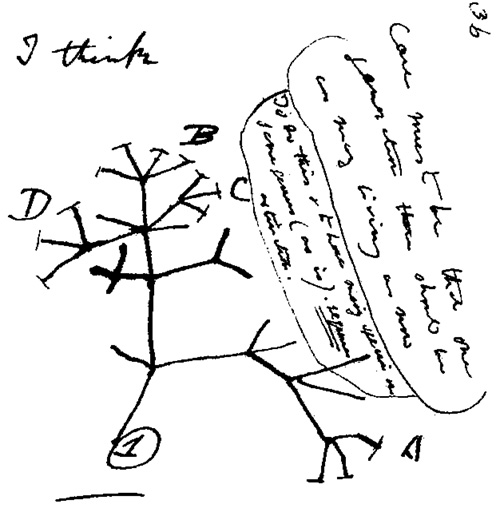
\includegraphics[scale=0.45]{gfx/darwin_tree.jpg}
	\end{center}
	\caption{
		"Drevo življenja", prva skica evolucijske zgodovine, narisal jo je 
		Charles Darwin leta 1837~\cite{cd}.
	}
	\label{img-darwin-tree}
\end{figure}

Spoznali bomo teoretično ozadje konstrukcije asimetričnega srednjega drevesa, nato pa bo 
sledila predstavitev programskega paketa Biopython, v katerega smo
vključili implementacijo asimetričnega srednjega drevesa, in ostalih orodij, ki smo
jih pri tem uporabili. Uspešnost implementirane metode bomo eksperimentalno ocenili
na treh vhodnih množicah, ki izražajo različne lastnosti, in na eni realni vhodni 
množici. Rezultate bomo primerjali s tremi popularnimi konsenznimi metodami glede
na razrešenost končnega drevesa in glede na Robinson-Fouldsovo metriko. 
Za  konec bomo preverili, za kakšno število dreves v vhodni množici je uporaba
implementirane metode še dovolj hitra, in predlagali možne izboljšave.


\chapter{Filogenetske in konsenzne metode}

V diplomski nalogi se povečamo konsenzni metodi asimetričnega srednjega drevesa. Da bi 
razumeli, zakaj so konsenzne metode v računski filogenetiki potrebne, bomo v tem 
razdelku zgolj na kratko predstavili, kako so filogenetska drevesa sploh zgrajena in 
kakšno vlogo pri tem igrajo konsenzne metode. 

\section{Filogenetske računske metode}

Filogenetske računske metode lahko razdelimo na dve večji skupini in sicer distančne in
statistične metode. Vse kot vhod prejmejo DNA- ali RNA-sekvence taksonomskih enot, 
katerih evolucijsko zgodovino želimo rekonstruirati, kot izhod pa vrnejo eno ali
več filogenetskih dreves, ki imajo konice (liste) označene z imeni taksonomskih enot.
Nekatere metode so zmožne oceniti tudi dolžino vej drevesa, pri čemer dolžina veje
predstavlja čas, ki je bil potreben za divergenco dveh taksonomskih enot iz skupnega
prednika. Izračun dolžin vej sicer ni odvisen zgolj od izbrane metode, temveč tudi 
od izbranega modela molekularne ure. Primere treh filogenetskih dreves za pet 
taksonomskih enot prikazuje slika \ref{img-input-trees}. Drevesa na sliki imajo 
dolžine vseh vej enake, med sabo pa se razlikujejo po topologiji.

\begin{figure}
	\begin{center}
		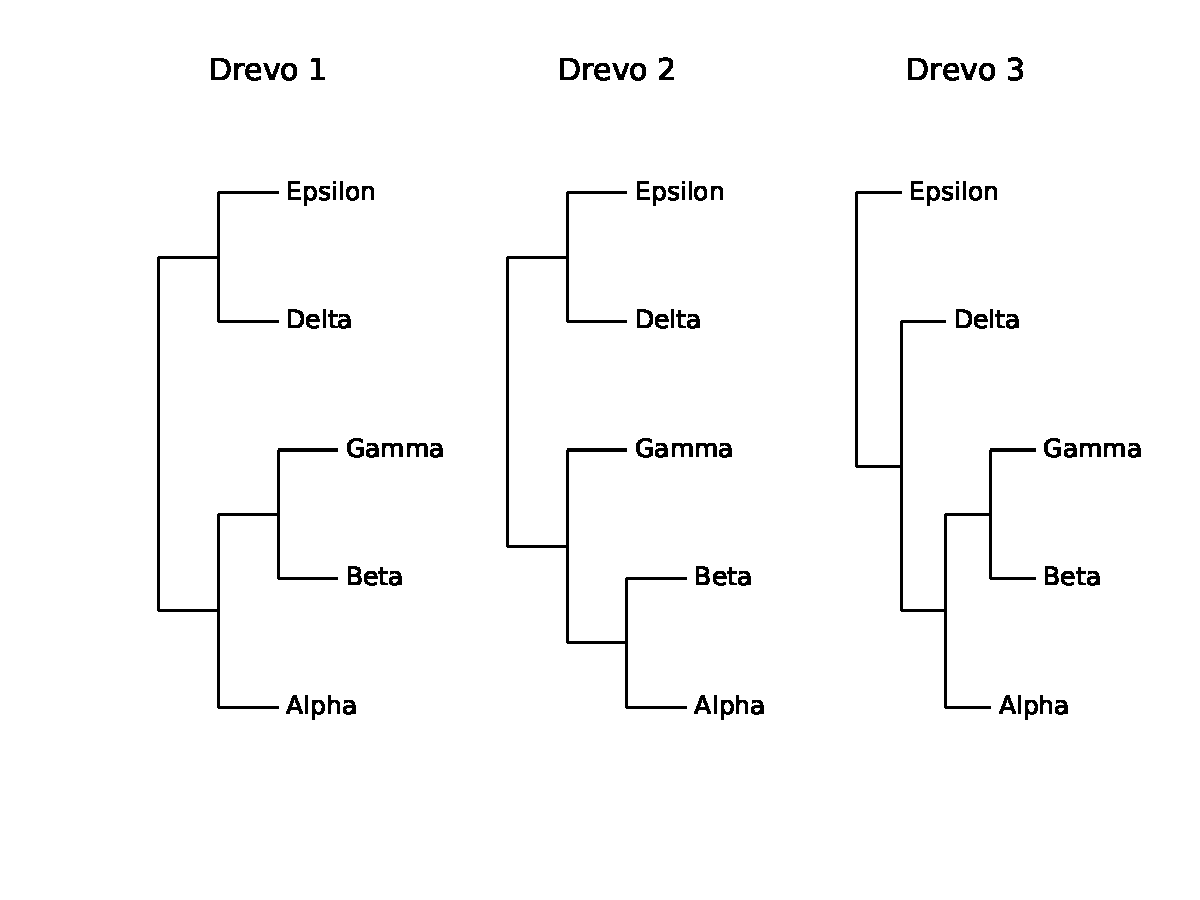
\includegraphics[scale=0.7, clip=true, trim=0 3cm 0 9mm]{gfx/input_trees_ex.pdf}
	\end{center}
	\caption{Primer treh filogenetskih dreves z različnimi topologijami.}
	\label{img-input-trees}
\end{figure}

\subsection{Distančne metode}
Distančne metode iz vhodnih sekvenc DNA ali RNA s pomočjo izbranega evolucijskega 
modela najprej generirajo distančno matriko, v kateri so zapisane razdalje med 
vsemi pari sekvenc. Razdalje predstavljajo divergentne čase med dvema taksonomskima 
enotama, zato evolucijske modele lahko uporabimo tudi v kombinaciji z drugimi 
metodami za izračun dolžin vej filogenetskega drevesa. Za generiranje distančne 
matrike imamo na voljo več različnih evolucijskih modelov, med njimi:
	\begin{itemize}
		\item Jukes-Cantor (JC69) je najbolj enostaven model, ki predpostavlja, 
			  da je frekvenca vseh nukleotidov enaka in da so vse možne 
			  substitucije na enem baznem paru enako verjetne~\cite{jc},
		\item Kimura (K80) model, ki substitucije baznega para razlikuje glede 
			  na tip in upošteva, da se lahko določen tip substitucije pojavi 
			  bolj pogosto~\cite{k80}. Tipe substitucij delimo na tranzicije 
			  (sprememba purina v purin ali sprememba pirimidina v pirimidin) 
			  ter transverzije (sprememba purina v pirimidina ali obratno)~\cite{fel},
		\item General Time Reversible (GTR) je najnaprednejši model, ki 
			  evolucijo modelira kot stohastični proces. Ne predpostavlja 
			  neodvisnosti vsek lokacij vhodnih sekvenc, temveč šteje frekvence 
			  pojavitve nukleotidov glede na pozicijo v kodonu. Nato oceni šest
			  parametrov, s pomočjo katerih zgradi matriko z verjetnostmi 
			  prehoda enega nukleotida v drugega~\cite{gtr}.
	\end{itemize}

\noindent Na podlagi razdalj, zapisanih v distančni matriki, izbrana metoda v gručo 
uvrsti po dve najbolj podobni taksonomski enoti hkrati (oz. povedano drugače, 
najbolj podobnima taksonomskima enotama določi skupnega prednika), dokler v 
gruče ne uvrsti vseh taksonomskih enot. Primera algoritmov, ki spadata v razred 
distančnih metod, sta UPGMA in metoda združevanja sosedov (angl., neighbor joining). 

\subsection{Metoda največje varčnosti}
Metoda največje varčnosti spada med starejše, vendar še vedno zelo uporabljane 
metode. Glavna ideja algoritma je analogna principu Occamovega rezila~-~med več 
medseboj tekmujočimi hipotezami evolucije izberemo tisto, ki minimizira število 
evolucijskih dogodkov. Metoda pregleda vsa potencialna drevesa in izbere tisto, 
ki vhodne sekvence lahko pojasni z najmanjšim številom potrebnih substitucij 
baznih parov. Tako drevo imenujemo najbolj varčno drevo 
(angl., most parsimonious tree)~\cite{parsimony}. Najbolj varčnih dreves je lahko
več, zato je izhodna množica najbolj varčnih dreves idealen primer vhodne množice 
za eno izmed metod za grajenje konsenznega drevesa.

\subsection{Metoda največjega verjetja}
Metoda maksimalnega verjetja (angl., maximum likelihood) je ena izmed statističnih
metod za grajenje filogenetskih dreves. Če za neko drevo predpostavimo, da predstavlja
pravilno evolucijsko zgodovino, potem njegovo verjetje predstavlja verjetnost 
pojavitve vhodnih sekvenc pri danem drevesu. Metoda poišče drevo, ki verjetje 
maksimizira in ob tem predpostavlja, da so verjetnosti substitucij na različnih 
baznih parih medsebojno neodvisne. Najprej izračuna kako verjetno je predlagano 
drevo za vsako lokacijo vhodnih sekvenc posebej, nato pa še produkt teh vrendosti, 
ki predstavlja končno verjetje drevesa. Verjetje drevesa ne predstavlja verjetnosti, 
da je to drevo dejansko pravilno. 

\subsection{Bayesova inferenca}
Bayesova inferenca je še en statistični pristop k iskanju filogenetskega drevesa. 
Zamisli o uporabi Bayesovega teorema so se pojavile že konec šestdesetih let, 
vendar do nedavnega implementacija takih algoritmov ni bila smiselna zaradi velike
računske zahtevnosti. Od metode maksimalnega verjetja se razlikuje zaradi uporabe 
vnaprej izbrane apriorne porazdelitve verjetnosti dreves~\cite{fel}. Stroka ima 
zaradi tega sicer deljena mnenja o primernosti uporabe, vendar s tem pridobimo 
lepo lastnost, in sicer zmožnost interpretacije rezultata kot porazdelitev 
verjetnosti dreves glede na vhodne sekvence.

\subsection{Vzorčenje primerov}

Ker nobena izmed metod ne zagotavlja pravilno generirane evolucijske zgodovine 
oz. pravilnosti ne moremo preveriti (razen v primeru laboratorijskih organizmov, 
kjer je razmerje vnaprej znano)~\cite{phy}, raziskovalci ponavadi uporabijo eno 
izmed metod vzorčenja primerov, npr. metoda izloči enega (angl., jackknife) ali 
metoda razmnoževanja primerov (angl., bootstrap), s katero vzorčijo 
lokacije vhodnih sekvenc in za vsak vzorec zgradijo svoje filogenetsko drevo. 
Vsako drevo, zgrajeno iz vzorca, se primerja s prvotno pridobljenim in izračuna 
se delež dreves, ki vsebujejo veje prvotnega drevesa. S pomočjo teh deležev 
lahko ocenimo, kolikšna je negotovost prvotno izračunane topologije 
filogenetskega drevesa~\cite{fel}.   

Težava metod ponovnega vzorčenja je, da ocenjujejo zgolj negotovost v okviru 
ene metode. Raziskovalci lahko pridobijo več nasprotujočih si hipotez o evolucijski 
zgodovini, naj si bo z uporabo različnih metod za računanje filogenetskega drevesa 
ali iz različnih virov podatkov. Ob tem se pojavi potreba po eni hipotezi o evoluciji, 
ki bi kar se da dobro zajemala vse evolucijske dogodke, ki jih nosijo med sabo 
tekmujoče si hipoteze. To lahko dosežemo z uporabo konsenznih metod.

\section{Konsenzne metode}
Konsenzne metode nad filogenetskimi drevesi so uporabljene po vsakem filogenetskem
algoritmu, ki kot izhod proizvede več filogenetskih dreves. Načeloma lahko delujejo 
nad katero koli množico dreves, v kateri imajo drevesa enake množice oznak listov. 
V tem se bistveno razlikujejo od metod super-dreves, katere so sposobne kombinirati 
tudi drevesa, katerih množice oznak listov niso enake~\cite{bw}. Poleg metode 
asimetričnega srednjega drevesa, ki jo obravnavamo v nadaljevanju tega dela, 
naštejmo nekatere najbolj pogoste konsenzne metode:

\begin{itemize}
	\item kompatibilno drevo je sestavljeno iz delov vseh vhodnih dreves; ni 
		  nujno, da za vhodno množico dreves kompatibilno drevo dejansko tudi 
		  obstaja~\cite{pw},
	
	\item striktni konsenz je najbolj konzervativna metoda, saj v končnem 
		  drevesu ohrani le tiste dele dreves, ki so prisotni v vseh drevesih 
		  vhodne množice~\cite{bw}. Primer striktnega konsenznega drevesa za 
		  vhodna drevesa iz slike \ref{img-input-trees} je prikazan na sliki 
		  \ref{img-strict-majority-amt-example},
	
	\item večinski konsenz vsebuje le tiste dele drevesa, ki so prisotni v več
		  kot polovici dreves vhodne množice~\cite{bw}. Primer večinskega 
		  konsenznega drevesa za vhodna drevesa iz slike \ref{img-input-trees} 
		  je prikazan na sliki \ref{img-strict-majority-amt-example},
	
	\item srednji konsenz oz. mediana je drevo, ki minimizira vsoto simetričnih 
	      razlik glede na drevesa v vhodni množici. Večinsko drevo je prav tako 
	      srednje drevo, kar pomeni, da vedno obstaja vsaj eno srednje drevo~\cite{pw}.
	
	\item adamov konsenz je drevo, ki ohrani strukturo poddreves, prisotnih v vseh 
	      vhodnih drevesih. Vedno obstaja, vendar lahko vsebuje poddrevesa, ki niso 
	      prisotna v nobenem drevesu vhodne množice~\cite{classification}.
	      
	\item Nelson-Pageva konsenza metoda je bila osnovana na ideji, da se eno drevo 
		  lahko moti, dve drevesi pa ne. Predpostavlja, da so deli dreves, prisotni
		  v dveh ali več vhodnih drevesih, zelo verjetno resnični. Take dele imenujemo 
		  replicirane komponente. Nelson-Pagevo drevo je tako drevo, ki vsebuje vse 
		  replicirane komponente vhodne množice in vse preostale dele dreves vhodne
		  množice, ki so z repliciranimi komponentami kompatibilni~\cite{classification}.  
\end{itemize}

\begin{figure}[h!]
	\begin{center}
		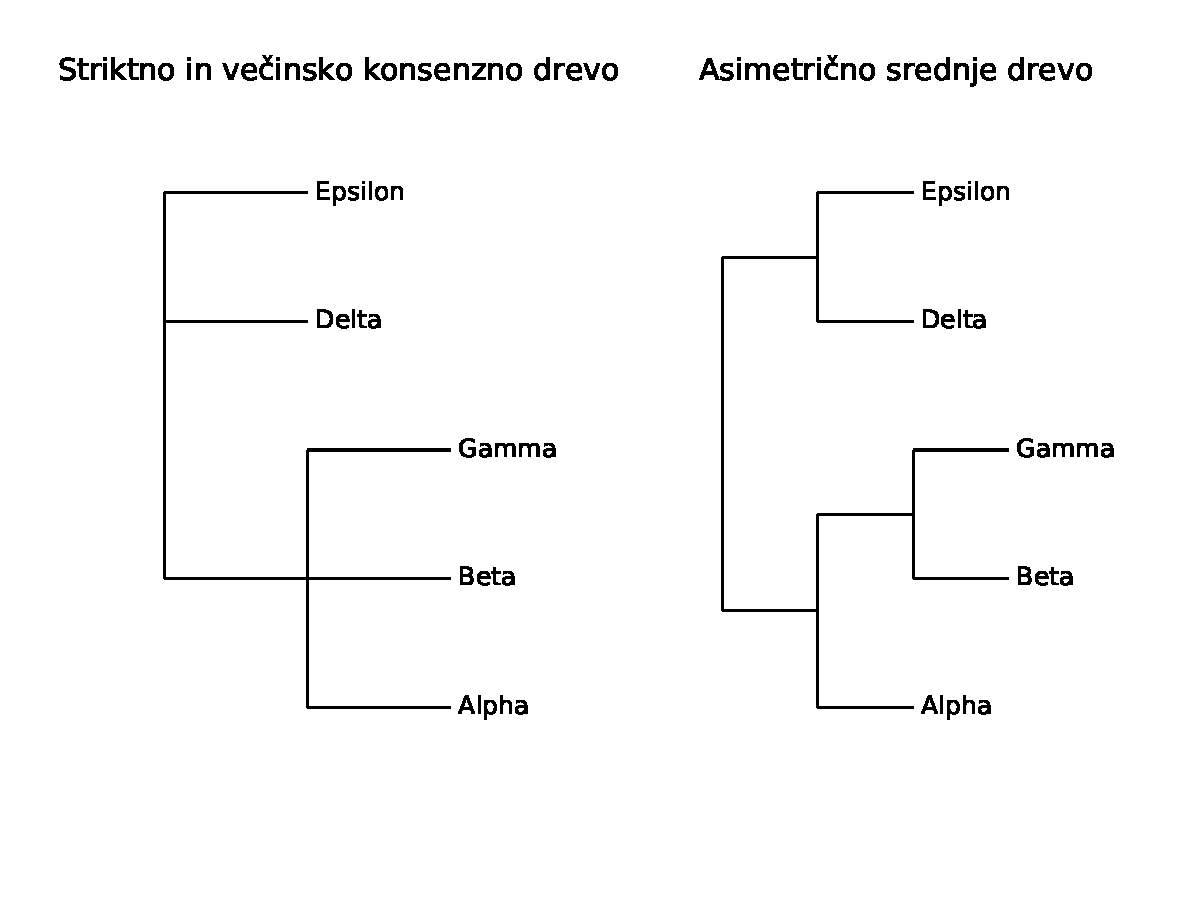
\includegraphics[scale=0.65, clip=true, trim=0 3cm 0 9mm]{gfx/strict_majority_amt_ex.pdf}
	\end{center}
	\caption{
		Na levi strani je prikazano striktno in večinsko konsenzno drevo za vhodna 
		drevesa iz slike \ref{img-input-trees}. Drevesi sta v tem primeru enaki. 
		Na desni je za isto vhodno množico prikazano asimetrično srednje drevo.
	}
	\label{img-strict-majority-amt-example}
\end{figure}

\noindent Večina konsenznih metod ignorira dolžine vej v vhodnih drevesih, tudi če so te navedene. 
Namen konsenznih metod je torej pridobiti topologijo drevesa, s katero se čim bolj strinjajo 
vhodna drevesa, ne pa tudi usklajevanje divergentnih časov taksonomskih enot in njihovih 
skupnih prednikov.  

\section{Programska oprema za izračun filogenetskih dreves}
Vse zgoraj opisane metode so že implementirane v samostojnih programskih paketih. Med najbolj znane spadajo:

\begin{itemize}
	\item ClustalW2 Phylogeny, ki omogoča izračun filogenetskega drevesa s 
		 pomočjo distančnih metod UPGMA in združevanja sosedov, korekcijo 
		 razdalj pa lahko opravi s pomočjo evolucijskega modela K80~\cite{clustalw2}. 
	      Poleg možnosti samostojne namestitve ga lahko uporabljamo tudi 
	      preko spletnega vmesnika, dostopnega na 
	      \url{http://www.ebi.ac.uk/Tools/phylogeny/clustalw2_phylogeny/}.
	\item PHYLIP, paket samostojnih programov, ki ponuja izračun filogenetskih dreves 
		  s pomočjo distančnih metod, metode največje varčnosti in metode največjega 
		  verjetja. Poleg tega ponuja programe za vzorčenje primerov ter program
	      za izračun konsenznega drevesa s pomočjo striktnega in večinskega konsenza. 
	      Korekcije razdalj je mogoče opraviti z evolucijskimi modeli JC69, K80 in F84~\cite{phylip}.
	\item MrBayes, ki izračun filogenetskega drevesa opravi s pomočjo bayesove inference. 
		  Za izračun posteriorne verjetnostne porazdelitve uporablja markove verige v 
		  kombinaciji z Metropolis-Hastingsovim algoritmom za učinkovito preiskovanje 
	      prostora topologij. Ker na izhodu proizvede mnogo dreves, ponuja tudi 
	      izračun konsenznega drevesa s pomočjo metode večinskega konsenza~\cite{mrbayes}.
	\item MEGA6, eno najbolj celovitih programskih okolij za izračun filogenetskih 
		  dreves, med drugim ponuja poravnavanje sekvenc pred njihovo uporabo z 
		  distančnimi metodami, metodami največje varčnosti ali metode maksimalnega
	       verjetja. Ponuja široko paleto evolucijskih modelov z izjemo modela GTR, 
	       izračun konsenznih dreves s pomočjo striktnega ali večinskega konsenza 
	       in možnost ponovnega vzorčenja. Program MEGA6 lahko uporabljamo preko ukazne
	       vrstice, vse funkcionalnosti pa so podprte tudi preko grafičnega vmesnika~\cite{mega6}. 
	\item HashCS, program za izračun konsenza filogenetskih dreves, ki se šteje za 
		  enega najhitrejših programov te vrste. Implementira lastni algoritem, ki 
		  teče v polinomskem času. Ker je bil izdelan z namenom hitrejšega povzemanja 
		  dreves, ki so rezultat enega izmed algoritmov z uporabo bayesove inference, 
		  predpostavlja, da je število vhodnih dreves mnogo večje kot število 
		  taksonomskih enot~\cite{hashcs}.
\end{itemize} 

\chapter{Asimetrično srednje drevo}
Metoda asimetričnega srednjega drevesa je nastala ob opažanju, da navadno srednje 
drevo kaznuje tiste dele dreves, ki ne nastopajo vsaj v polovici dreves vhodne množice, 
čeprav bi bilo smotrno, da se uporabi kar se da veliko informacije iz vseh vhodnih 
dreves~\cite{pw}.

Metoda kot vhod prejme množico $k$ filogenetskih dreves 
$T = \left\{ {T_1, T_2, ..., T_k} \right\}$, katera imajo liste označene z $n$ 
taksonomskimi enotami iz množice $S = \left\{ {s_1, s_2, ..., s_n} \right\}$. 
Sledijo naslednji koraki algoritma, katerega dele bomo podrobneje obravnavali
 v naslednjih poglavjih:
\begin{itemize}
	\item drevesa pretvorimo v primerno reprezentacijo,
	\item poiščemo nekompatibilne pare poddreves in konstruiramo graf nekompatibilnosti,
	\item v grafu nekompatibilnosti poiščemo največjo neodvisno množico vozlišč,
	\item rekonstruiramo drevo iz vozlišč največje neodvisne množice.
\end{itemize}

\section{Kodiranje dreves}
Izbira predstavitve drevesa je pomembna za njihovo nadaljno manipulacijo. Izhajamo iz 
opažanja, da vsaka povezava v drevesu (rob), $e \in E(T_i)$, drevo razdeli na dva dela oz. particiji.
 Do vsakega lista (taksonomske enote $s$) vodi enolična pot, predstavljena z množico 
 robov, ki na tej poti nastopajo. Označimo jo s $\pi(s)$. Nato definiramo preslikavo 
 dveh argumentov (\ref{eq:1}), ki zavzame vrednost 1 v kolikor pot do podanega lista 
 poteka preko podanega roba, sicer pa 0. $c(e, s)$ za vsak rob $e \in E(T_i)$ torej 
 definira biparticijo drevesa $T_i$~\cite{pw}. V prvi množici so listi, do katerih 
 lahko pridemo, če pot vodi preko roba $e$, v drugi pa tisti, do katerih v tem 
 primeru ne moremo.

\begin{align}
	c(e, s) = 
	\left\{
		\begin{array}{ll}
			1 & e \in \pi(s) \\
			0 & e \notin \pi(s)
		\end{array}
	\right.
	\label{eq:1}
\end{align}

Vsak rob drevesa določa poddrevo, to pa predstavlja skupnega prednika s svojimi 
potomci. Takemu poddrevesu pravimo tudi klad (taksonomsa skupina, angl., clade). Ne bo nas zanimala 
celotna struktura poddreves, temveč zgolj njihovi listi. Vsak klad drevesa lahko 
predstavimo z binarnim nizom, ki ga dobimo z uporabo preslikave \ref{eq:2}, pri 
čemer je potrebno povdariti, da je vrstni red posameznih znakov v binarnem nizu 
pomemben, saj je na vsak znak vezan pomen; vsako posamezno mesto v nizu pripada 
enemu izmed listov drevesa, znak na tem mestu pa zgolj indicira prisotnost ali
neprisotnost lista oz. taksonomske enote v kladu, kodiranem z binarnim nizom.


\begin{align}
	c_e = \left\{ c(e, s): s \in S \right\} \label{eq:2}
\end{align}

V kolikor binarne nize vseh kladov drevesa zberemo v množico (\ref{eq:3}), 
nam $C(T_i)$ določa kodiranje celotnega drevesa $T_i$. Primer dveh takih množic
je prikazan na sliki \ref{img-bistring-trees-example}, kjer so binarni nizi 
prikazani na vejah, ki vodijo do korenov kladov.

\begin{align}
	C(T_i) = \left\{ c_e : e \in E(T_i) \right\} \label{eq:3}
\end{align}

Kodiranje sedaj lahko izvedemo nad vsemi drevesi vhodne množice $T$, pri čemer je 
ponovno potrebno poudariti, da se pomen posameznih mest v binarnih nizih med 
različnimi drevesi ne sme spreminjati, saj sicer kladov iz različnih dreves ne 
bi mogli medsebojno primerjati. 

\begin{figure}
	\begin{center}
		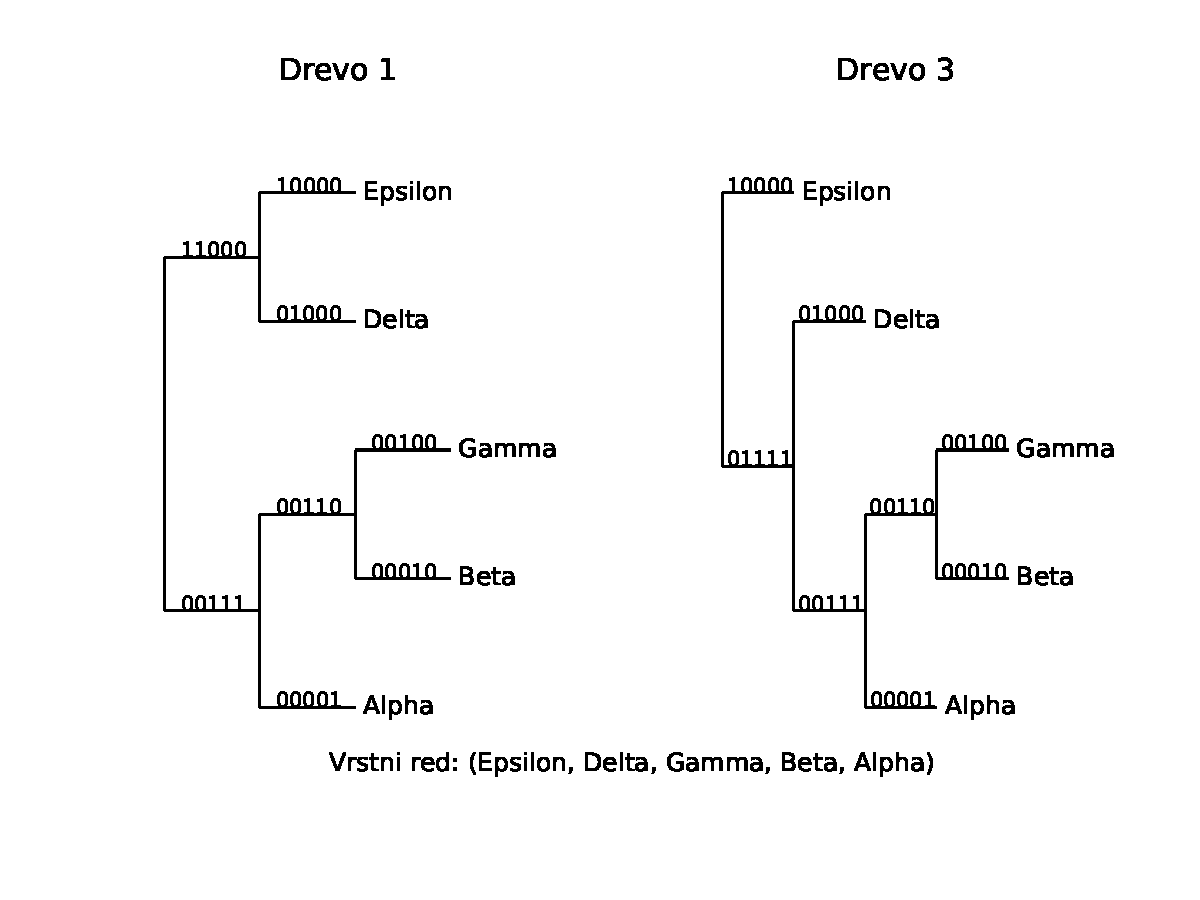
\includegraphics[scale=0.7, clip=true, trim=0 2cm 0 9mm]{gfx/bitstring_trees.pdf}
	\end{center}
	\caption{Vsi binarni nizi za prvo in tretje drevo iz slike \ref{img-input-trees}.}
	\label{img-bistring-trees-example}
\end{figure}

\section{Kompatibilnost binarnih nizov} 
Za konstrukcijo grafa nekompatibilnosti najprej potrebujemo kriterij kompatibilnosti 
kladov oz. binarnih nizov, ki jih kodirajo. Za potrebe lažje predstavitve 
kompatibilnosti za vsak binarni niz $c_e$ definiramo množico $\phi(c_e)$ (\ref{eq:4}), 
ki vsebuje oznake taksonomskih enot, prisotnih v kladu oz. njegovem pripadajočem 
binarnem nizu $c_e$. 

\begin{align}
	\phi(c_e) = c_e^{-1}(1) = \left\{ s \in S: c(e, s) = 1 \right\} \label{eq:4} \\
	\phi(j) \cap \phi(k) = \emptyset \lor \phi(j) \subseteq \phi(k) \lor \phi(k) \subseteq \phi(j) \label{eq:5}
\end{align} 

Če za binarna niza $j$ in $k$ iz poljubnih dveh dreves vhodne množice $T$ velja 
pogoj~\ref{eq:5}, potem sta binarna niza kompatibilna. Vennov diagram pripadajočih 
množic $\phi(j)$ in $\phi(k)$ prikazuje slika \ref{img-venn-compatibility}. 
V kolikor velja $\left|\phi(j)\right| = 1$ ali $\left|\phi(k)\right| = 1$, potem 
sta binarna niza $j$ in $k$ vedno kompatibilna.   

\begin{figure}
	\begin{center}
		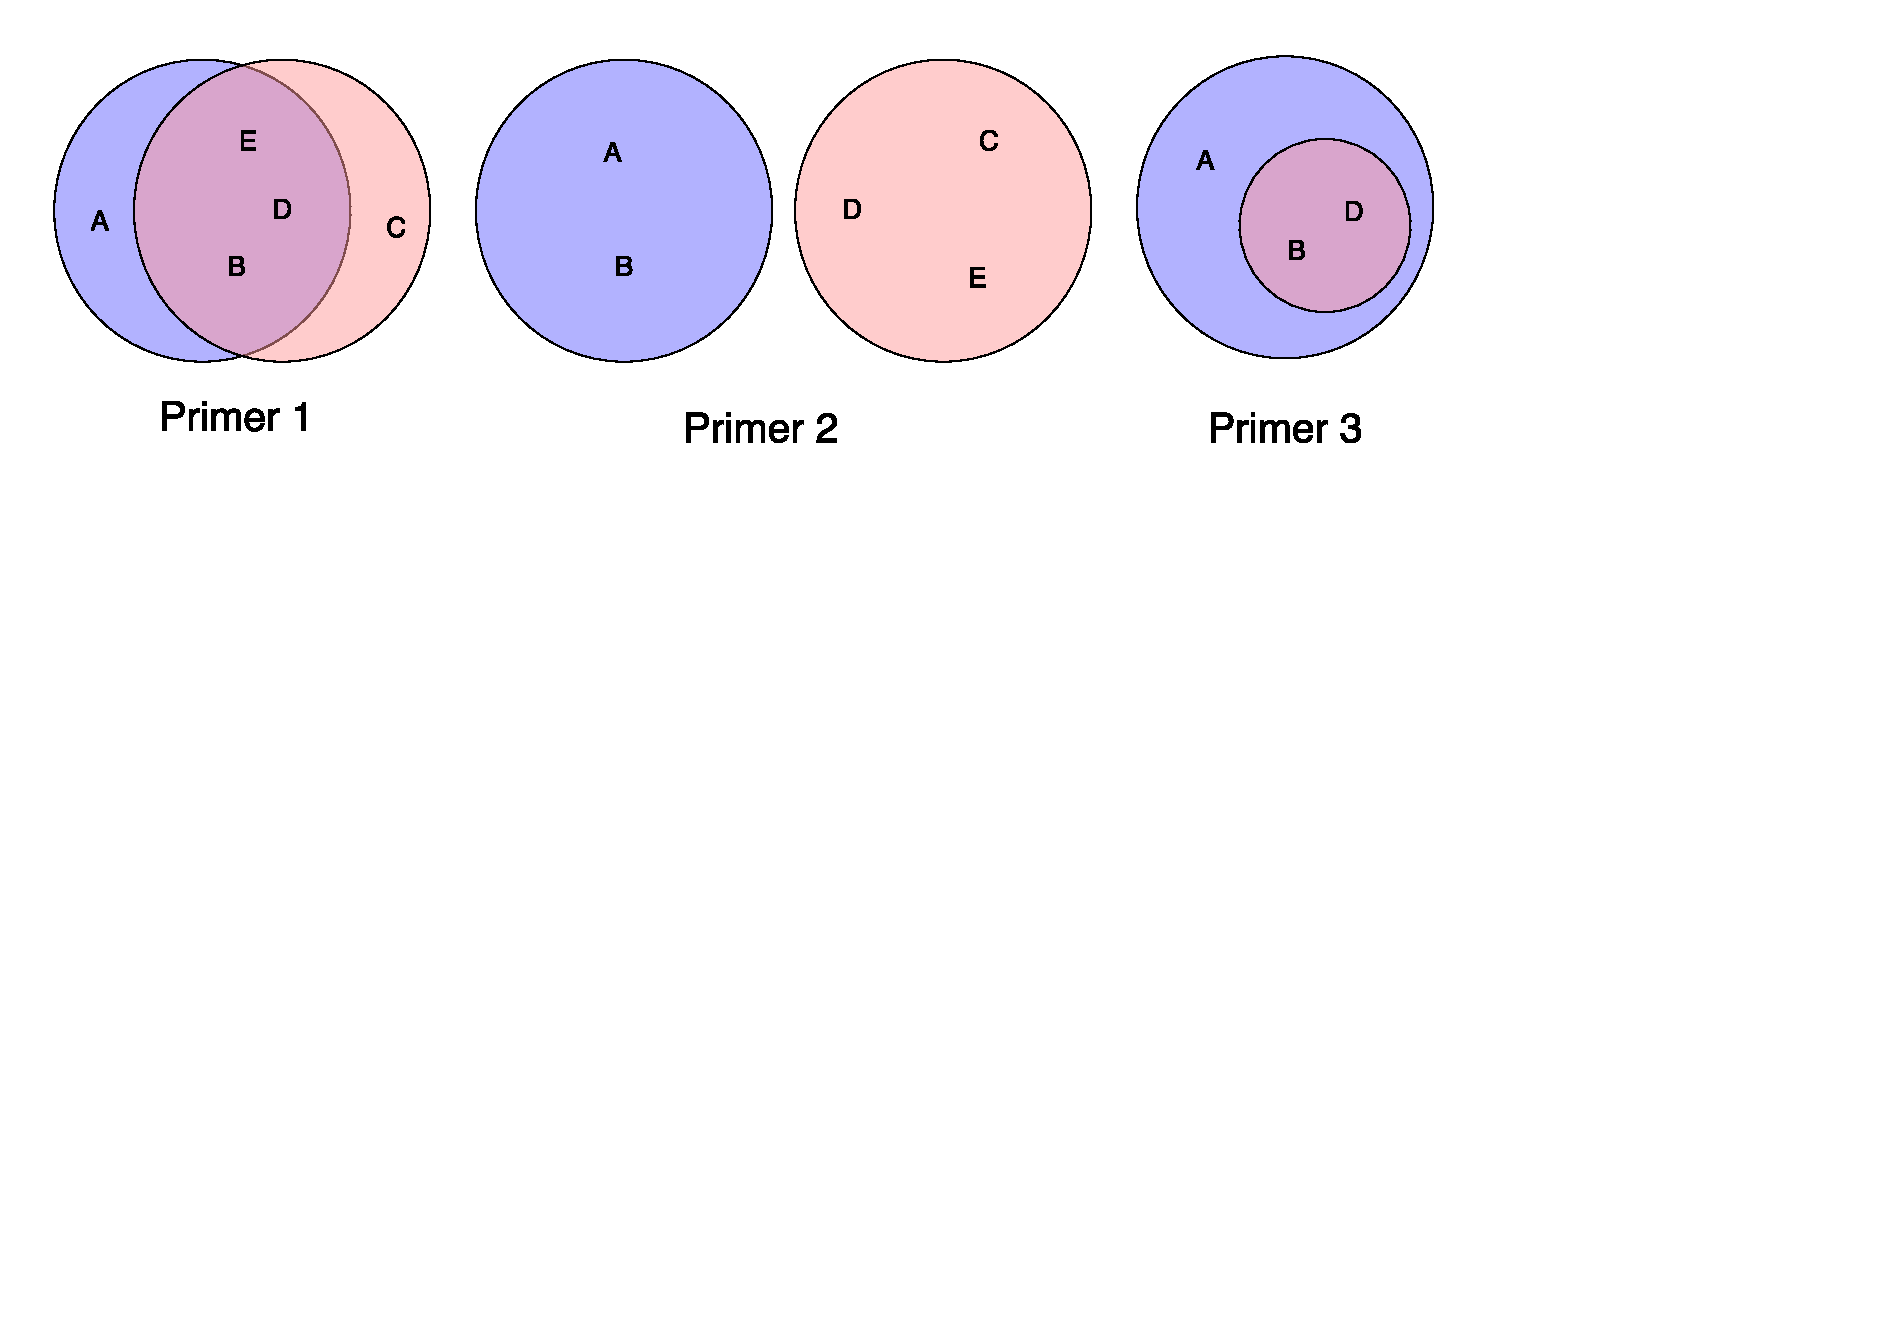
\includegraphics[scale=0.54, clip=true, trim=0 15cm 0 0]{gfx/venn-amt-compatibility.pdf}
	\end{center}
	\caption{
		Primera 2 in 3 prikazujeta kompatibilni množici $\phi$, v primeru 1 pa 
		sta množici nekompatibilni.
	}
	\label{img-venn-compatibility}
\end{figure}

V kolikor kompatibilnost kladov interpretiramo v smislu filogenetskega drevesa, 
potem posamezen klad predstavlja poddrevo s korenom, ki je notranje vozlišče 
drevesa $T_i$. Notranje vozlišče filogenetskega drevesa predstavlja skupnega 
prednika vsem vozliščem v poddrevesu pod njim. Nekompatibilni sta tisti poddrevesi, 
ki trdita, da se je iz obeh skupnih prednikov razvilo nekaj skupnih taksonomskih 
enot, a je hkrati v vsaj enem poddrevesu prisotna taksonomska enota, ki je v drugem 
poddrevesu ni. V tem primeru poddrevesi torej ponujata nasprotujoči si informaciji
o evolucijski zgodovini. 

\section{Graf nekompatibilnosti}
Z uporabo kriterija nekompatibilnosti binarnih nizov lahko zgradimo graf 
nekompatibilnosti $I(V_1, V_2, ..., V_k, E) = I(V, E)$. Vsaka množica vozlišč 
$V_i$ predstavlja binarne nize $C(T_i)$, povezave v grafu pa vzpostavimo med 
tistimi vozlišči, katerih pripadajoči binarni nizi so med sabo 
nekompatibilni~\cite{pw}. S povezovanjem vozlišč označimo binarne nize, ki v 
končnem drevesu skupaj ne morejo biti prisotni, sicer bi filogenetsko drevo 
podajalo dvoumne informacije o evolucijski zgodovini. 

Graf nekompatibilnosti vseh treh vhodnih dreves iz slike \ref{img-input-trees} 
je prikazan na sliki \ref{img-incompat-graph-example}. V prvem in drugem drevesu 
sta medsebojno nekompatibilna klada $(Gamma, Alpha)$ in $(Gamma, Beta)$. Drevesi 
ponujata nasprotujoči si informaciji - prvo za najbolj sorodno taksonomski 
enoti $Gamma$ ponuja taksonomsko enoto $Alpha$, drugo pa taksonomsko enoto $Beta$. 
Prvo in drugo drevo imata medsebojno kompatibila klada $(Epsilon, Delta)$, ki pa 
sta nekompatibilna s kladom $(Delta, Gamma, Beta, Alpha)$ iz tretjega vhodnega 
drevesa. Medtem ko prvo in drugo drevo trdita, da imata taksonomski enoti 
$Epsilon$ in $Delta$ neposrednega skupnega prednika, tretje drevo temu nasprotuje.

\begin{figure}
	\begin{center}
		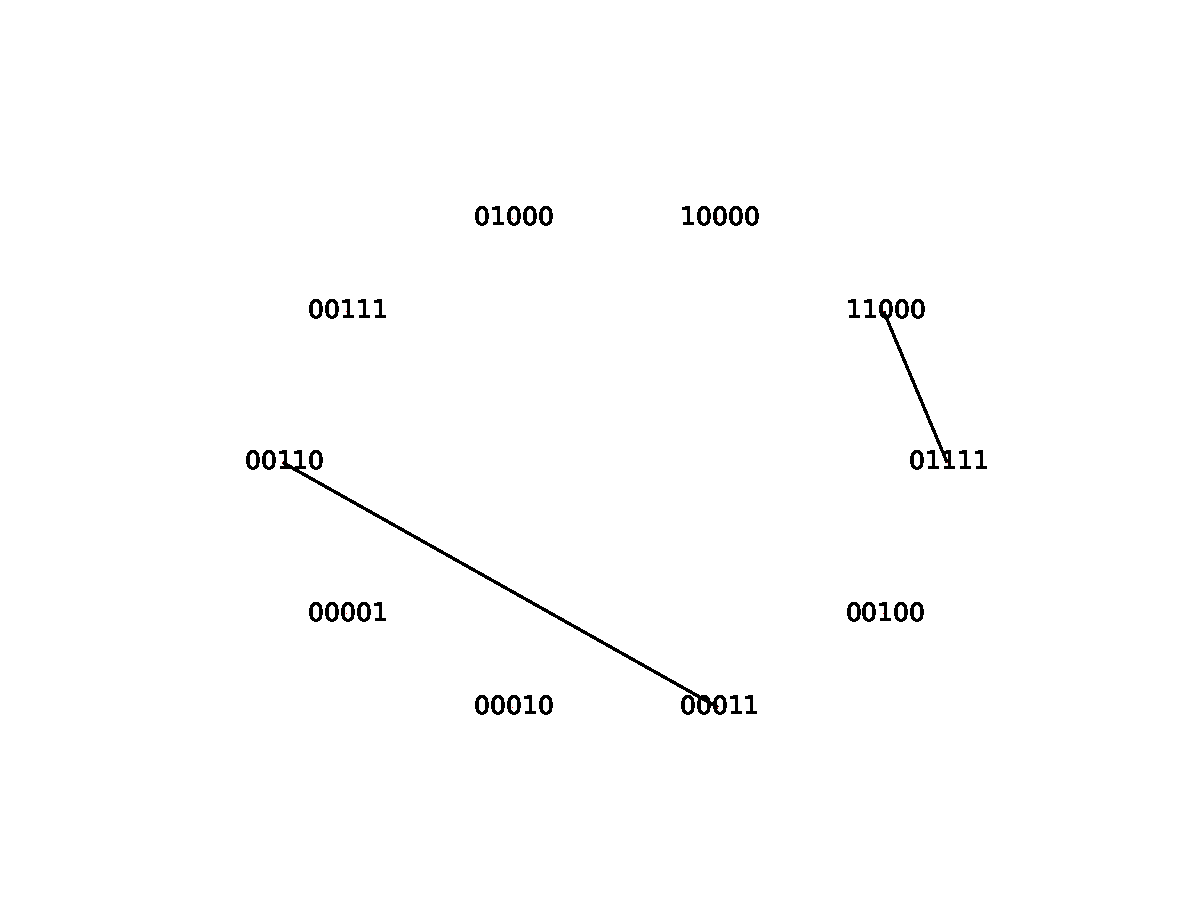
\includegraphics[scale=0.7, clip=true, trim=2cm 2cm 2cm 2cm]{gfx/incompat_graph.pdf}
	\end{center}
	\caption{
		Graf nekompatibilnosti bitnih nizov za vhodna drevesa iz 
		slike~\ref{img-input-trees}. Vozlišča predstavljajo unikatne binarne 
		nize iz vseh dreves vhodne množice $T$, povezave pa so vzpostavljene 
		med pari vozlišč, katerih binarni nizi medsebojno niso kompatibilni.
	}
	\label{img-incompat-graph-example}
\end{figure}

\section{Največja neodvisna množica}
Graf nekompatibilnosti vsebuje vse informacije, ki jih potrebujemo za izbiro 
binarnih nizov, ki bodo prisotni v končnem filogenetskem drevesu. Vanj želimo 
vključiti kar se da veliko informacij, prisotnih v drevesih vhodne množice $T$. 
Najprej je potrebno zagotoviti, da vključimo binarne nize, ki so skupni vsem 
vhodnim drevesom $T_i$ (drevo, ki bi vsebovalo le te binarne nize, bi bilo 
striktno konsenzno drevo). Obenem želimo vključiti čimveč preostalih binarnih 
nizov, vendar ne takih, da bi bil katerikoli par nekompatibilen. 

Matematično orodje, ki nam iz grafa $I(V, E)$ omogoča izbiro vozlišč, ki paroma 
ne bodo kršile pogoja nekompatibilnosti, se imenuje neodvisna množica 
(angl., independent set). Neodvisna množica grafa je katerakoli množica vozlišč 
$V_{Indep} \subseteq V$, med katerimi ni medsebojnih povezav. Največja neodvisna 
množica grafa (angl., maximum independent set - MIS) je tista neodvisna množica 
$V_{MIS} \subseteq V$, ki vsebuje največ vozlišč. Potrebno je povdariti, da za 
nek graf $I(V, E)$ lahko obstaja več različnih $V_{MIS}$. Ker vozlišča $V_{MIS}$ 
predstavljajo binarne nize oz. klade končnega drevesa, to pomeni, da za en graf 
$I(V, E)$ lahko obstaja več asimetričnih srednjih dreves. Primeri
vseh največjih neodvisnih množic za graf nekompatibilnosti iz 
slike~\ref{img-incompat-graph-example} so narisani na 
sliki~\ref{img-mis-examples}.

\begin{figure}
	\begin{center}
		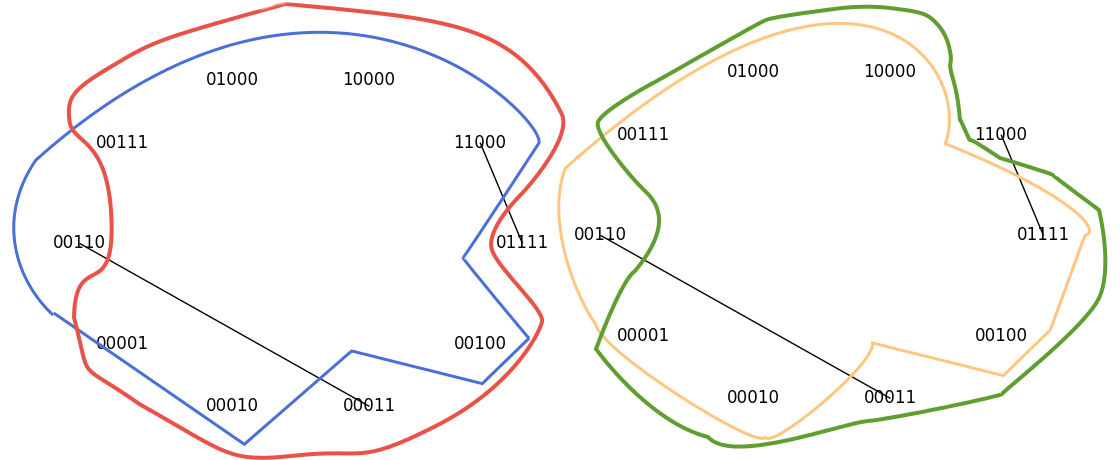
\includegraphics[scale=0.43]{gfx/incompat_graph_all.png}
	\end{center}
	\caption{
		Vse štiri različne največje neodvisne množice za graf nekompatibilnosti 
		iz slike~\ref{img-incompat-graph-example}.
	}
	\label{img-mis-examples}
\end{figure}

Vozlišča grafa $I(V, E)$, katerega sestavimo iz $k$ dreves vhodne množice $T$, 
sestavljajo neodvisne množice $V_1, V_2, ..., V_k$. Vozlišča znotraj ene množice
nikoli niso medsebojno povezana, saj njihovi pripadajoči binarni nizi pripadajo 
istemu drevesu. Vozlišči iz različnih množic pa lahko tvorita povezavo, v kolikor 
sta nekompatibilni. Tak graf imenujemo tudi k-partitni graf. Za bipartitne grafe 
obstaja trivialen polinomski algoritem s časovno zahtevnostjo $O(n^2)$, v splošnem 
pa problem največje neodvisne množice za k-partitne grafe sodi v razred 
NP-težkih algoritmov~\cite{pw}. 

\section{Rekonstrukcija drevesa}
S tem, ko smo določili največjo neodvisno množico $V_{MIS}$ grafa $I(V, E)$, 
smo določili klade končnega drevesa, katerega strukturo pa je potrebno še 
rekonstruirati iz izbranih binarnih nizov. Problem rekonstrukcije evolucijske 
zgodovine $n$ taksonomskih enot iz njihovih binarnih nizov je dobro znan in se 
imenuje problem filogenije. Zanj obstaja algoritem s časovno kompleksnostjo $O(nm)$, 
pri čemer je $n$ število taksonomskih enot, $m$ pa število binarnih nizov v največji
 neodvisni množici~\cite{gd}.

Najprej kreiramo matriko M dimenzij $n×m$. Binarne nize, ki pripadajo vozliščem 
množice $V_{MIS}$ kot stolpce zložimo v matriko $M$. Nato stolpce interpretiramo 
kot števila v binarnem zapisu, jih pretvorimo v desetiško obliko in sortiramo. 
Odstranimo stolpce s podvojeno vrednostjo, tako da ostanejo le stolpci z unikatnimi 
števili. S tem pridobimo matriko $M'$.

\begin{figure}
	\begin{center}
		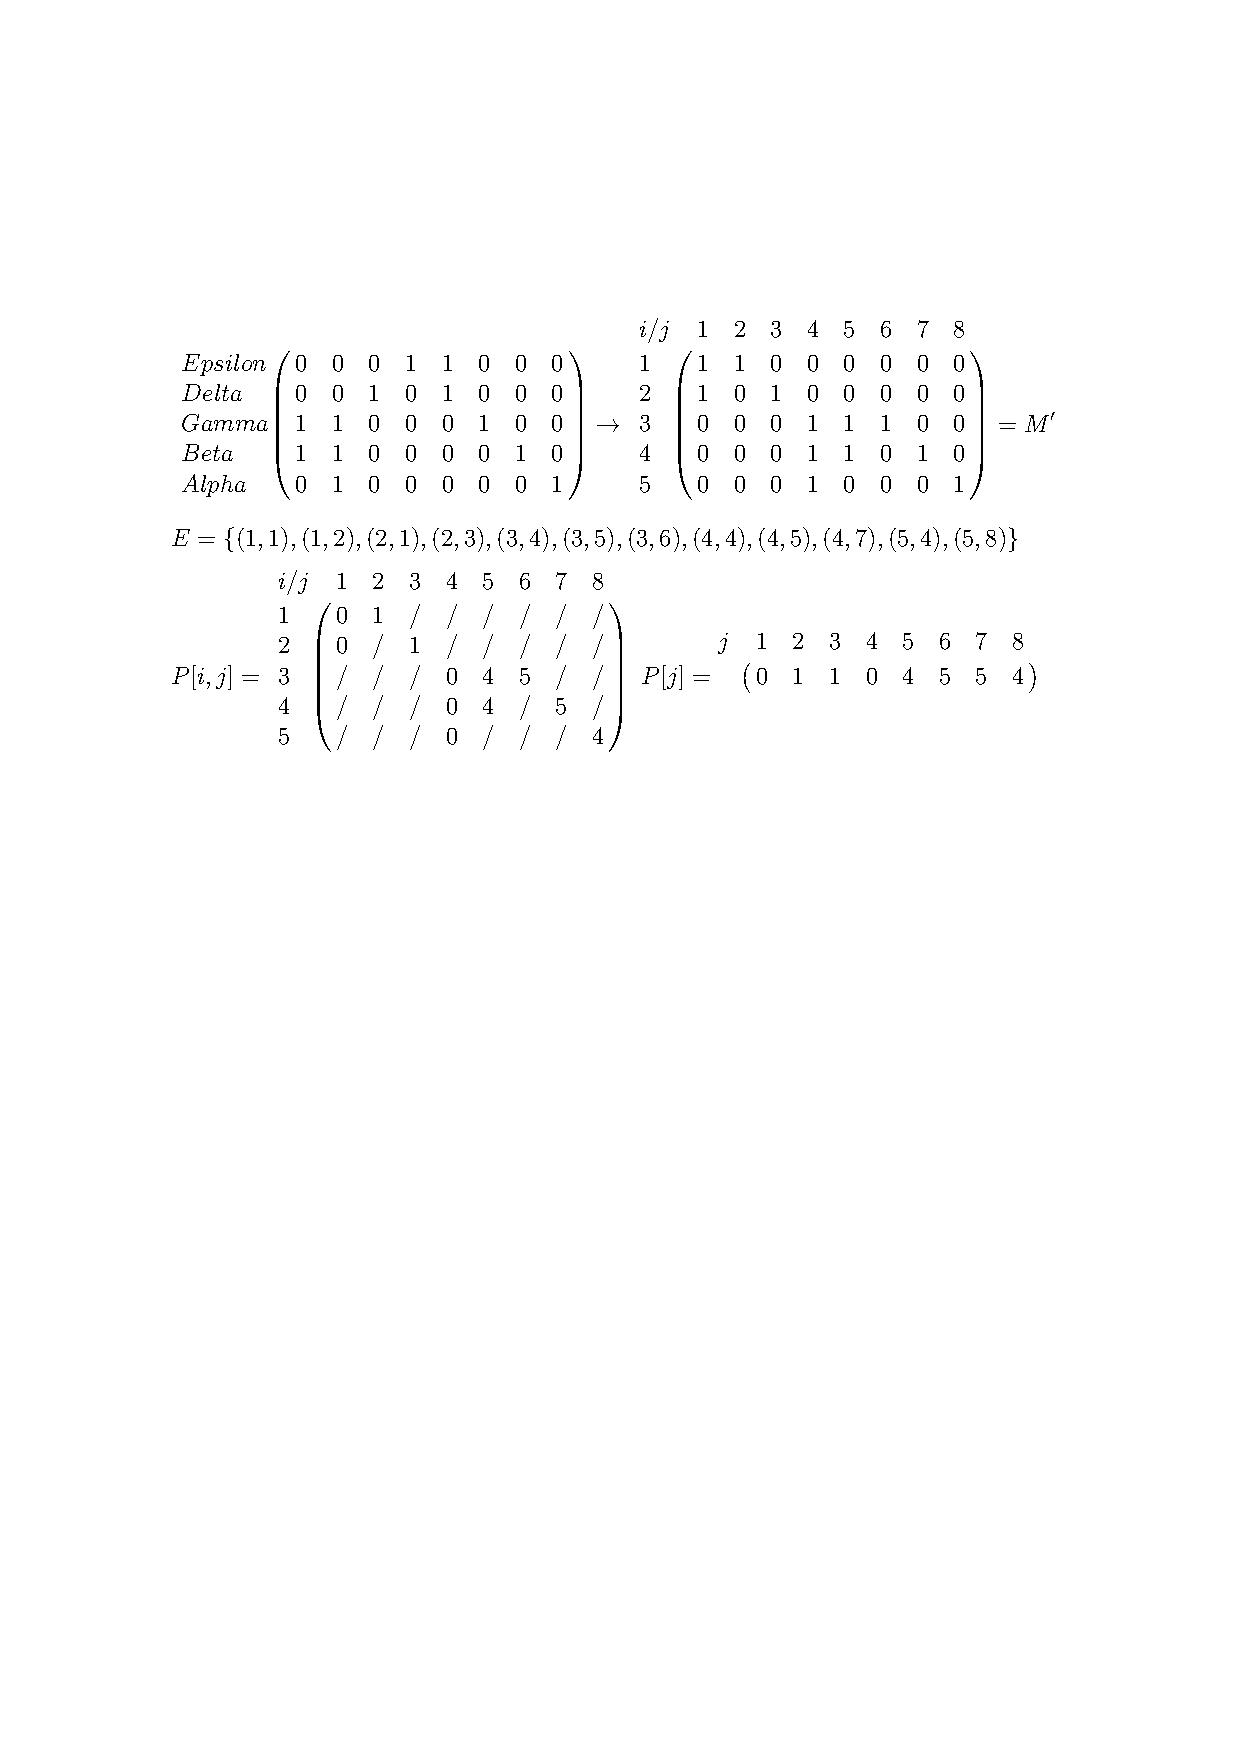
\includegraphics[scale=0.8, clip=true, trim=2.9cm 17cm 3cm 5cm]{gfx/tree_reconstruction_m.pdf}
	\end{center}
	\caption{
		Primer izračuna matrike $M'$, množice parov indeksov $E$ in vseh 
		vrednosti $P(i, j)$ ter $P(j)$ za prvo največjo neodvisno množico iz 
		slike~\ref{img-mis-examples}. Ker enačba~\ref{eq:9} v tem primeru 
		velja, iz matrike $M'$ lahko zgradimo filogenetsko drevo.
	}
	\label{img-reconstruct-m}
\end{figure}

Naj bo $I_i$ množica indeksov vrstic, $I_j$ pa množica indeksov stolpcev matrike 
$M'$. Množica $E$ (\ref{eq:6}) predstavlja vse pare indeksov 
$(i, j) \in I_i \times I_j$ matrike $M'$, katerih vrednost je enaka ena.

\begin{align}
	E = \left\{ {(i, j): i \in I_i, j \in I_j, M'(i, j) = 1} \right\} \label{eq:6} \\
	P(i, j) = 
		\left\{
		\begin{array}{ll}
			\max(\left\{k: (i, k) \in E, k < j\right\}) \\
			0 $      "ce tak $k$ ne obstaja$
		\end{array}
		\right.
	\label{eq:7}
\end{align}

Vsak par $(i, j) \in E$ predstavlja klad $j$, v katerem je prisotna taksonomska
enota $i$. Za vsak tak par poiščemo vrednost $P(i, j)$, ki ustreza indeksu klada
$k$, v katerem je vsebovan klad $j$ (\ref{eq:7}), pri čemer tudi klad $k$ vsebuje
taksonomsko enoto $i$. V kolikor tak klad ne obstaja, to pomeni, da ima klad $j$
svoj koren pozicioniran najbolj blizu korena celotnega končnega drevesa izmed vseh
kladov s prisotno taksonomsko enoto $i$. 

Ko imamo poračunane vse vrednosti $P(i, j)$, lahko za vsak $j \in I_j$ poiščemo
vrednost $P(j)$(\ref{eq:8}). Ta predstavlja najvišji indeks klada, v katerem je
klad $j$ vsebovan. Ker so kladi sortirane padajoče glede na njihove desetiške
vrednosti, najvišji indeks pravzaprav pomeni, da iščemo očeta klada $j$, ki je
na čim nižjem nivoju v končnem drevesu, tako da je klad $j$ še v celoti vsebovan.
	
\begin{align}
	P(j) = \max(\left\{P(i, j): (i, j) \in E\right\}) \label{eq:8} \\
	P(i, j) = P(j)   ~~~~~~~~~~~~  \forall (i, j) \in E \label{eq:9}
\end{align}

\begin{figure}[h!]
	\begin{center}
		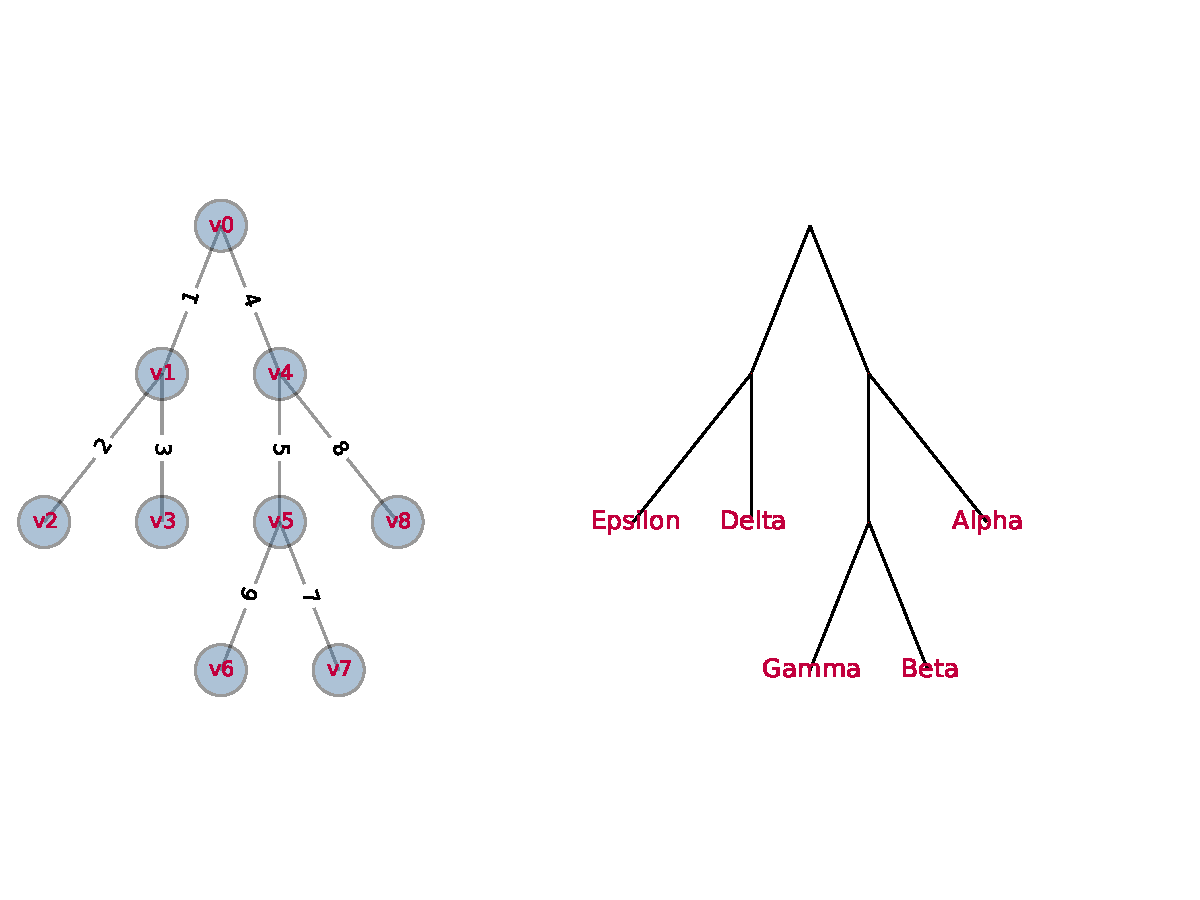
\includegraphics[scale=0.67, clip=true, trim=0 3cm 3cm 3cm]{gfx/tree_reconstruct_1.pdf}
	\end{center}
	\caption{
		Na levi strani je prikazan graf, ki je rekonstruiran iz vrednosti 
		$P[j]$ iz slike \ref{img-reconstruct-m}. Da iz grafa pridobimo 
		končno drevo, prikazano na desni strani, za označevanje listov 
		uporabimo matriko $M'$ iz slike \ref{img-reconstruct-m}.
	}
	\label{img-reconstruct-1}
\end{figure}

V kolikor velja enačba \ref{eq:9}, potem za matriko $M'$ obstaja filogenetsko 
drevo~\cite{gd}. V tem primeru se lahko lotimo njegove konstrukcije. Najprej 
ustvarimo graf, v katerega kot vozlišča dodamo koren bodočega drevesa $r$ in za 
vsak $j \in I_j$ svoje vozlišče $v_j$. Nato za vsako vozlišče $v_j$, za katerega 
velja $P(j) > 0$, ustvarimo povezavo $(v_{P(j)}, v_j)$ in povezavo označimo z $j$. 
Vsa preostala vozlišča $v_j$, za katere velja $P(j) = 0$, povežemo s korenom 
drevesa s pomočjo povezave $(r, v_j)$, in prav tako označimo z $j$. Primer takega
grafa, konstruiranega za matriko $M'$ iz slike \ref{img-reconstruct-m} je prikazan
na levi strani slike \ref{img-reconstruct-1}. Tak graf je že drevo, vendar je potrebno 
razrešiti oznake na povezavah.

Ker vsaka vrstica matrike $M'$ predstavlja eno taksonomsko enoto, lahko oznake povezav
določimo tako, da pregledujemo matriko po vrsticah. Za vsak $i \in I_i$ najdemo največji 
$j$, za katerega velja $M'(i, j) = 1$. Dobljeni $j$ nam predstavlja oznako povezave, 
na koncu katere je prisoten list, kateremu dodelimo oznako taksonomske enote trenutne
vrstice $i$. To storimo za vse vrstice, s čimer označimo vse liste. Kot prikazuje 
primer dokončanega drevesa na desni strani slike \ref{img-reconstruct-1}, za konec 
notranjim vozliščem in povezavam odstranimo oznake. S tem smo prišli do končnega 
filogenetskega drevesa, ki ga označimo s $\tau$.  

\section{Vrednost asimetričnega srednjega drevesa}
Omenili smo že, da za en graf nekompatibilnosti lahko obstaja več največjih 
neodvisnih mnnožic in da to pomeni, da lahko sestavimo več različnih 
asimetričnih srednjih dreves. Prvotni razlog za uporabo konsenznih metod 
je iz večih dreves pridobiti eno drevo, zato potrebujemo metriko, s pomočjo 
katere se bomo lahko odločili za eno, najbolj podprto drevo.  

Najprej uvedemo utež binarnega niza $w(c_e)$~(\ref{eq:10}), ki je preprosto 
število dreves v vhodni množici $T$, ki vsebujejo binarni niz $c_e$. Vrednost 
asmetričnega srednjega drevesa $\tau$ glede na vhodno množico $T$ je 
določena~(\ref{eq:11}) kot vsota uteži binarnih nizov, ki so prisotni v 
asimetričnem srednjem drevesu, vendar niso prisotni v vseh vhodnih drevesih 
(oz. striktnem konsenznem drevesu)~\cite{pw}.

\begin{align}
	w(c_e) = \left| \left\{ i: c_e \in C(T_i) \right\} \right| \label{eq:10} \\
	value(T, \tau) = \sum_{c \in C(\tau) - \cap C(T_i)} w(c) \label{eq:11}
\end{align}

Najboljše najdeno asimetrično srednje drevo je tisto, ki maksimizira dano vsoto 
uteži~\ref{eq:11}.

\section{Aproksimacijski algoritmi}
Ker je problem konstrukcije asimetričnega srednjega drevesa polinomsko prevedljiv 
na problem največje neodvisne množice~\cite{pw} in zato za več kot dve drevesi 
sodi v razred NP-težkih problemov, je lahko izvajanje algoritma prepočasno, če 
imamo veliko dreves v vhodni množici $T$. Zato si bomo ogledali dva 
aproksimacijska algoritma, ki imata polinomsko časovno zahtevnost.

Prvi, $\frac{2}{k}$-aproksimacijski algoritem, je enostaven. Za vsak par dreves 
$T_i, T_j \in T$ izračunamo asimetrično srednje drevo $\tau_{ij}$ in izberemo 
tistega, ki maksimizira vrednostno funkcijo $value(T, \tau_{ij})$. Ker je tako 
asimetrično srednje drevo sestavljeno iz dveh dreves, posledično lahko vsebuje 
le klade, ki so prisotni v teh dveh drevesih.

V kolikor imajo drevesa vhodne množice $T$ veliko skupnih kladov, je primernejši 
drugi algoritem. Naj bo $V^* \subseteq V$ podmnožica vozlišč grafa nekompatibilnosti 
$I(V, E)$, in sicer tistih, ki so skupna vsem drevesom. Takih vozlišč v naslednjem 
koraku ne potrebujemo, saj niso povezana z nobenim drugim vozliščem. Nato izračunamo 
največje ujemanje (angl., maximum matching) v grafu $I(V - V^*, E)$, s čimer pridobimo 
množico robov $E_{M} \subseteq E$, ki nimajo skupnih vozlišč~\cite{mgt}. 
Vozlišča $V_{M}$, ki so krajišča robov iz množice $E_{M}$, odstranimo iz množice $V$ 
in ostanejo nam le neujemajoča vozlišča $V_{N} = V - V_{M}$. Primer iskanja množice 
$V_N$ je prikazan na sliki \ref{img-maxmatch}. Iz binarnih nizov, pripadajočih 
vozliščem množice $V_{N}$, rekonstruiramo asimetrično srednje drevo po običanjem 
postopku. Tako drevo, za razliko od drevesa izračunanega s pomočjo prvega 
aproksimacijskega algoritma, lahko vsebuje klade iz večih dreves vhodne 
množice hkrati~\cite{pw}. 

\begin{figure}
	\begin{center}
		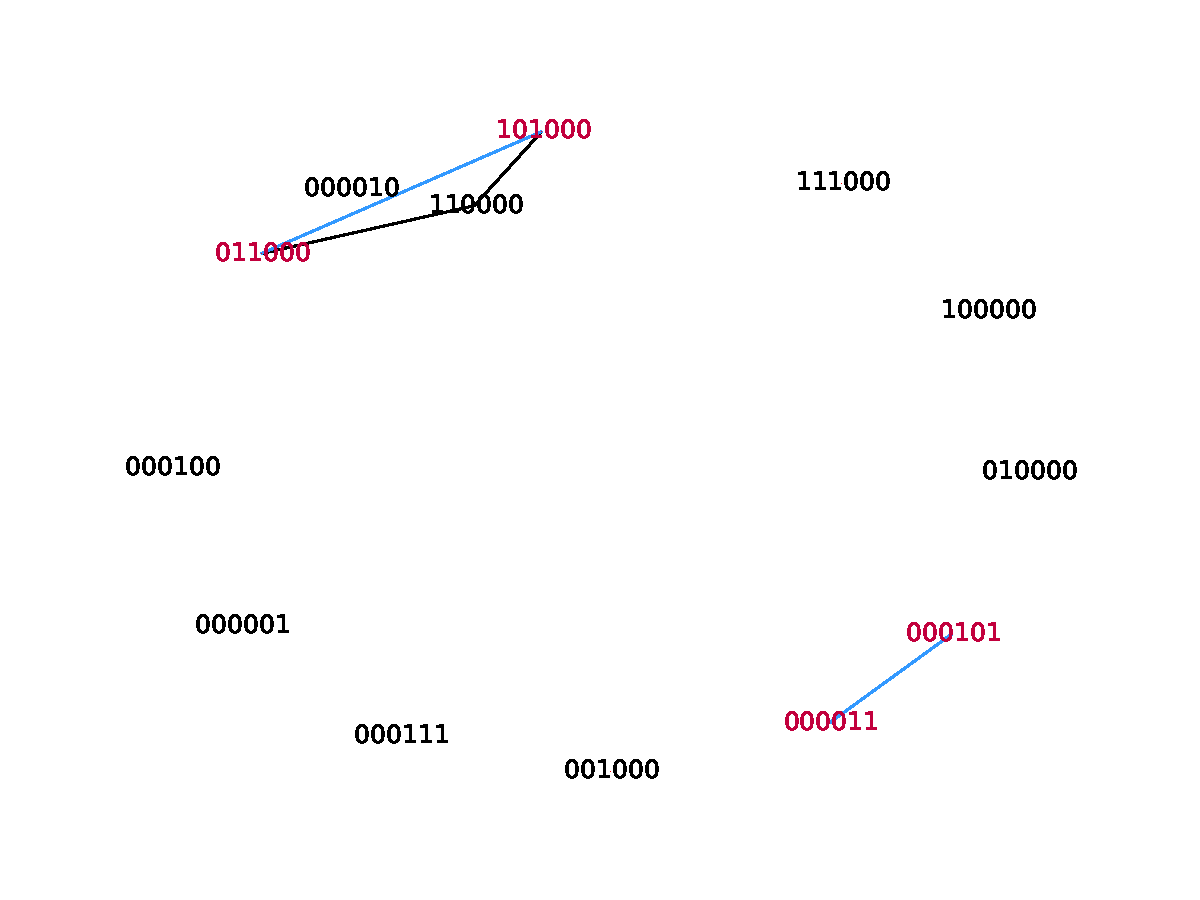
\includegraphics[scale=0.65, clip=true, trim=2cm 1cm 1cm 2cm]{gfx/maxmatch_graph.pdf}
	\end{center}
	\caption{
		Primer računanja bitnih nizov asimetričnega srednjega drevesa s pomočjo 
		največjega ujemanja. Robovi, ki spadajo v množico največjega ujemanja 
		$E_{M}$ so obarvani modro, njihova krajišča pa rdeče. Vsi bitni nizi, 
		ki so obarvani črno, sestavljajo končno drevo.
	}
	\label{img-maxmatch}
\end{figure}

\chapter{Implementacija algoritma}

\section{Biopython}
Biopython~\cite{biopython} je odprtokodni paket modulov, napisan v programskem 
jeziku Python, ki ponuja mnoge funkcionalnosti s področja bioinformatike. 
Olajša nam delo s formati datotek, kot so BLAST, ClustalW, FASTA ter GenBank
in ponuja enostaven dostop do spletnih storitev, npr. NCBI. 
Poleg funkcionalnosti, implementiranih v programskem jeziku Python ponuja
tudi enostaven dostop do zunanjih programov. Nekateri glavni moduli paketa 
Biopython, ki so relavantni tudi za računanje filogenetskih dreves, so: 

\begin{itemize}
	\item $Bio.SeqIO$: razredi, ki nam omogočajo branje, pisanje in 
	      manipuliranje sekvenc v različnih formatih ($FASTA$, $Nexus$, ...),
	\item $Bio.AlignIO$: razredi, ki nam omogočajo branje, pisanje in
	      manipuliranje poravnanih sekvenc,
	\item $Bio.Application$: razredi, s pomočjo katerih enostavno dostopamo
	      do zunanje namenske programske opreme, kot npr. PhyML in RAxML
	\item $Bio.Phylo$: razredi in funkcije za izračun filogenetskih dreves
\end{itemize} 

Modul $Bio.Phylo$ že omogoča izračun filogenetskih dreves s pomočjo 
metod UPGMA, Neighbor Joining in Maximum Parsimony. Poleg tega ponuja 
tudi metode ponovnega vzorčenja bootstrap in jackknife.  

Izračun konsenznih filogenetskih dreves je mogoč s pomočjo podmodula 
$Bio.Phylo.Consensus$ v katerem so bile najprej implementirane metode 
striktnega, večinskega in adamovega konsenza, sedaj pa izračun lahko 
opravimo tudi s pomočjo metode asimetričnega srednjega drevesa. Branje 
in pisanje dreves je že omogočeno za formate Newick, CDAO in PhyloXML. 
Modul ponuja tudi vmesno reprezentacijo drevesa, ki ga uporabljamo med 
izračunom in ni vezan na končni format.

\section{Podrobnosti implementacije}
Glavna entiteta, ki je nastopala v obravnavi metode asimetričnega srednjega 
drevesa je bil bitni niz. Zato je pomembno, da zanj uporabimo primerno hitro 
podatkovno strukturo. Razred, ki podatkovno strukturo že implementira se 
imenuje $\_BitString$, prebiva pa v podmodulu $Bio.Phylo.Consensus$. 
$\_BitString$ razširja Pythonovo vgrajeno podatkovno strukturo $String$, 
zato ga lahko uporabljamo na enak način. Med operatorji, ki jih lahko izvajamo 
nad podatkovno strukturo, so konjunkcija, disjunkcija in ekskluzivna 
disjunkcija nad posameznimi mesti, vsebuje pa tudi metodi za preverjanje 
vsebovanosti enega bitnega niza v drugem in preverjanje kompatibilnosti 
dveh binarnih nizov. 

\subsection{Izračun največje neodvisne množice}
Modul $Bio.Phylo$ za izrisovanje filogenetskih dreves uporablja paket 
networkx\footnote{\url{https://networkx.github.io/}}. Ta poleg samega 
izrisovanja ponuja tudi konstrukcijo grafov in njihovo nadaljno 
manipulacijo. Na grafu zmore izračunati aproksimacijo največje neodvisne 
množice, a se s tem nismo mogli zadovoljiti, saj je bila aproksimacija že 
za majhna vhodna drevesa preveč nenatančna, da bi dobili uporaben rezultat. 
Na srečo je problem največje neodvisne množice polinomsko prevedljiv na 
problem največje klike v komplementarnem grafu, katero networkx zna poiskati.
Kljub temu se je iskanje vseh največjih klik komplementarnega grafa izkazalo 
za dokaj počasno. 

Ob opazovanju, da naš algoritem izrablja le eno procesorsko jedro, smo
se odločili, da lahko iskanje največje klike opravimo na vseh razpoložljivih 
procesorjih s pomočjo zunanjega programa Parallel Maximum Clique (PMC)~\cite{pmc},
v kolikor zaznamo prisotnost programa na uporabnikovem sistemu. Čeprav smo s tem
vnesli dodatno odvisnost od zunanje programske opreme, lahko odločitev utemeljimo
s precej večjo hitrostjo implementacije PMC v primerjavi z lastno implementacijo
v programskem jeziku Python. V kolikor program ni najden, se iskanje največjih 
klik kljub temu opravi z uporabo paketa networkx.

\subsection{Izračun največjega ujemanja v grafu}
Pri uporabi druge aproksimacijske metode za izračun asimetričnega 
srednjega drevesa ne računamo največje neodvisne množice, 
temveč največje ujemanje grafa. Paket networkx za reševanje 
problema vsebuje funkcijo {\it max\_weight\_matching()}, pri čemer 
so vse uteži robov grafa enake 1.

Tako kot natančna metoda, tudi prva aproksimacijska metoda v grafu
nekompatibilnosti išče največjo neodvisno množico. V kolikor bi za
obe metodi uporabili isti algoritem za iskanje največje neodvisne 
množice, bi bila prva aproksimacijska metoda mnogo počasnejša kot
je sicer lahko. Zato smo izkoristili dejstvo, da graf nekompatibilnosti
v tem primeru sestavljata le dve particiji. Za tak graf obstaja
polinomski algoritem~\cite{hopcroft-karp}, s pomočjo katerega 
lahko izračunamo največje ujemanje. Problem največjega ujemanja
je v polinomskem času prevedljiv v problem minimalnega pokritja 
bipartitnega grafa, ta pa v bipartitnih grafih predstavlja komplement 
maksimalne neodvisne množice. Programsko kodo, s katero smo največje
ujemanje bipartitnega grafa prevedli v vozlišča največje neodvisne
množice, prikazuje slika~\ref{code-mm-to-mvc-to-mis}.

\begin{figure}[h!]
\begin{python}
verts = graph.nodes()
top, bottom = nx.bipartite.sets(graph)
mates = nx.max_weight_matching(graph, maxcardinality=True)
matched = mates.keys()
top_unmatched = [v for v in top if v not in matched]
cwo = [
    adj for adj in graph[v] if adj in bottom
    for v in top_unmatched
]
cwo += top_unmatched
# minimalno pokritje
mvc = set(
    [v for v in top if v not in cwo] 
    + list(set(bottom) & set(cwo))
)
# maksimalna neodvisna mnozica
mis = [v for v in verts if v not in mvc]
\end{python}
\caption{
	Programska koda za prevedbo največjega ujemanja v bipartitnem 
	grafu v minimalno pokritje grafa in nato v maksimalno neodvisno 
	množico. 
}
\label{code-mm-to-mvc-to-mis}
\end{figure}

\subsection{Rekonstrukcija drevesa}
Za rekonstrukcijo drevesa smo potrebovali orodje, ki je zmožno dela z matrikami. 
Ker je paket Biopython že odvisen od paketa numpy\footnote{\url{http://www.numpy.org/}},
je ta bil logična izbira. Med kreiranjem matrike je bilo potrebno binarne nize 
pretvoriti v stolpce matrike. Za to potrebo smo razredu \_BitString dodali metodo 
$to\_numpy()$, katera niz ničel in enic pretvori v binarni vektor tipa 
$numpy.ndarray$ z eno dimenzijo. Za potrebe sortiranja smo razredu 
$\_BitString$ dodali še metodo $\_\_int\_\_()$, ki izračuna desetiško vrednost 
binarnega niza.

\subsection{Programski vmesnik}

Slika~\ref{code-amt-func} prikazje glavo implementirane funkcije, ki se nahaja v 
modulu {\it Bio.Phylo.Consensus}. Celotna koda je navedena v dodatku~\ref{appendix-code-amt_consensus}.
Metoda privzeto izračuna točno asimetrično srednje
drevo, vendar je računska kompleksnost za več kot dve drevesi eksponentna, zato 
lahko uporabnik, v kolikor to želi, z drugim parametrom izbere eno izmed 
aproksimacijskih metod. 

\begin{figure}[h!]
	\begin{python}
		def amt_consensus(trees, method='no_approx')
	\end{python}
	\caption{Glava funkcije za izračun asimetričnega srednjega drevesa iz modula {\it Bio.Phylo.Consensus}.}
	\label{code-amt-func}
\end{figure}

\noindent Metoda {\it Bio.Phylo.Consensus.amt\_consensus}
sprejema dva parametra:

\begin{itemize}
\item {\bf trees} je seznam objektov tipa {\it BaseTree.Tree}. Drevo je lahko v kateremkoli formatu, ki ga podpira Biopython.

\item {\bf method} je tipa {\it niz}, s katerim izbiramo metodo izračuna. Veljavne so tri vrednosti:

\begin{itemize}
    \item {\bf no\_approx} izračun točnega drevesa,

    \item {\bf bi\_approx} izračun s kombiniranjem največ dveh dreves,

    \item {\bf maxmatch\_approx} izračun drevesa s pomočjo največjega ujemanja.
\end{itemize}
\end{itemize}
    
\section{Enostaven primer uporabe}
Primer uporabe programske kode je najbolj enostavno prikazati najprej na
enostavnejšem primeru. Recimo, da imamo pripravljeno datoteko z imenom 
{\it primer\_a.tre} in vsebino na sliki \ref{trees-input}. Vsebuje pet dreves
v formatu Newick, iz katerih želimo izračunati asimetrično srednje drevo
in ga izrisati.

\begin{figure}[h!]
\begin{lstlisting}
             ((A, (B, C)), (D, (E, F)));
             ((B, (A, C)), (D, (E, F)));
             ((A, (B, C)), (E, (D, F)));
             ((B, (A, C)), (E, (D, F)));
             ((C, (B, A)), (E, (D, F)));
\end{lstlisting}
\caption{
	Primer petih polno razrešenih filogenetskih dreves s šestimi taksonomskimi 
	enotami, ki so kodirana v formatu Newick.
}
\label{trees-input}
\end{figure}

Uporaba konsenzne metode asimetričnega srednjega drevesa v paketu Biopython je 
enostavna. Slika~\ref{amt-example} predstavlja osnoven primer uporabe. V prvi 
vrstici uvozimo modul $Bio.Phylo$, v drugi iz podmodula $Bio.Phylo.Consensus$ 
uvozimo funkcijo $amt\_consensus$,  v tretji pa uvozimo paket za risanje $pyplot$.

\begin{figure}[h!]
	\begin{python}
		from Bio import Phylo
		from Bio.Phylo.Consensus import amt_consensus
		from matplotlib import pyplot
	
		trees = list(Phylo.parse('primer_a.tre', 'newick'))
		amt = amt_consensus(trees)
		amt.ladderize()
		Phylo.draw(amt)
		pyplot.show()
	\end{python}
	\caption{
		Primer programske kode za branje dreves iz datoteke in izračun 
		asimetričnega srednjega drevesa.
	}
	\label{amt-example}
\end{figure}


V peti vrstici uvozimo filogenetska drevesa iz datoteke $primer\_a.tre$ in jih 
razčlenimo, s čimer dobimo seznam objektov tipa $Bio.Phylo.BaseTree.Tree$. V 
šesti vrstici s preprostim klicem funkcije iz obstoječega seznama dreves 
izračunamo asimetrično srednje drevo. V sedmi vrstici drevo preoblikujemo tako, 
da bodo globlja poddrevesa prikazana na vrhu, in v zadnjih dveh vrsticah drevo 
izrišemo na ekran. 

Rezultat je programa iz figure \ref{amt-example} je prikazan na 
sliki~\ref{img-example-output}. Poleg drevesa so prikazane še osi, 
ki v našem primeru sicer niso pomembne, v splošnem pa iz osi x lahko 
razberemo divergentne čase taksonomskih enot. 
\\
\begin{figure}[h!]
	\begin{center}
		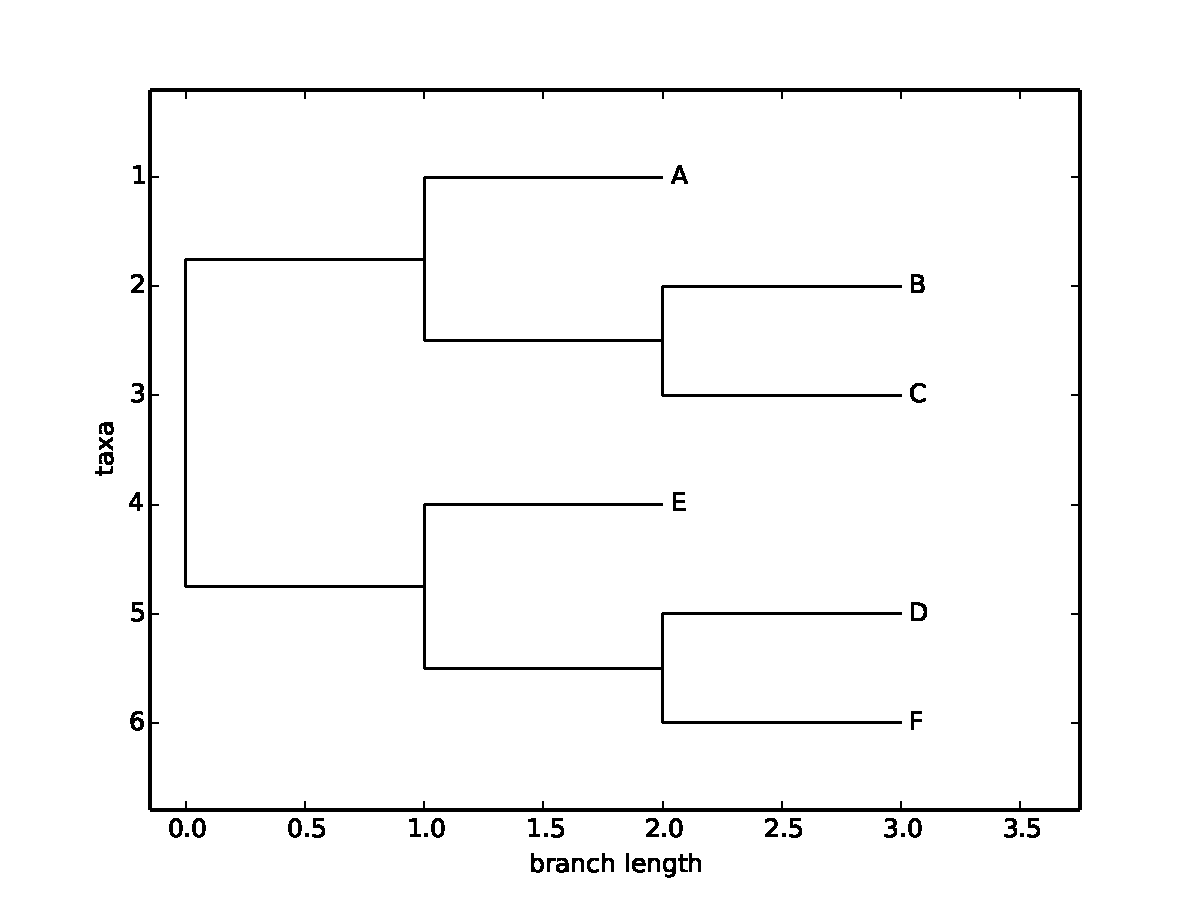
\includegraphics[scale=0.6, clip=true, trim=1cm 0 1cm 1cm]{gfx/ex_b.pdf}
	\end{center}
	\caption{Rezultat programa iz slike \ref{amt-example}.}
	\label{img-example-output}
\end{figure}

\section{Primer uporabe z grajenjem dreves iz sekvenc DNA}
V prejšnjem primeru uporabe smo filogenetska drevesa prebrali iz vnaprej pripravljene
datoteke. Običajno temu ni tako in je drevesa pred uporabo konsenzne
metode potrebno najprej izračunati. Primer programske kode, s katero v paketu
Biopython izračunamo filogenetska drevesa s pomočjo metod UPGMA, metode združevanja 
sosedov in metode največje varčnosti, iz njih pa tri konsenzna drevesa, 
prikazuje slika~\ref{phylo-trees-example}.

\begin{figure}
\begin{lstlisting}
              5   13
        Alpha     AACGTGGCCACAT
        Beta      AAGGTCGCCACAC
        Gamma     CAGTTCGCCACAA
        Delta     GAGATTTCCGCCT
        Epsilon   GAGATCTCCGCCC
\end{lstlisting}
\caption{
Vhodne sekvence DNA v datoteki {\it msa.phy}, ki je ena izmed testnih datotek
programskega paketa Biopython~\cite{bio-phylo}, v formatu, ki ga uporablja 
programski paket PHYLIP.
}
\end{figure}

Najprej v šesti vrstici s pomočjo modula {\it Bio.AlignIO} iz vhodne datoteke uvozimo
vnaprej poravnane sekvence DNA, ki pripadajo taksonomskim enotam. Nato v deseti vrstici
kreiramo objekt tipa {\it DistanceCalculator}, ki služi za izračun distančne matrike. Tega
potrebujemo v naslednjih dveh vrsticah, kjer kreiramo konstruktor dreves tipa 
{\it DistanceTreeConstructor} za metodo UPGMA in metodo združevanja najbližjih sosedov.
Metoda največje varčnosti za razliko od distančnih metod potrebuje objekt tipa
{\it ParsimonyScorer}, ki ga kreiramo v petnajsti vrstici, in preiskovalnik prostora 
dreves tipa {\it NNITreeSearcher}, ki ga kreiramo vrstico nižje. Oba objekta podamo
konstruktorju metode največje varčnosti v sedemnajsti vrstici.

Sedaj imamo pripravljeno vse, da lahko v vrsticah 20-24 s pomočjo prej ustvarjenih 
konstruktorjev dreves iz vhodnih sekvenc DNA zgradimo tri filogenetska drevesa. 
Nato v vrsticah 27-29 iz zgrajenih dreves izračunamo še konsenzna drevesa s 
pomočjo metod asimetričnega srednjega drevesa, večinskega konsenza in adamovega konsenza.
Tako kot v prvem primeru uporabe za konec izračunana konsenzna drevesa še izrišemo, 
kar naredimo s pomočjo paketa {\it pyplot}.


\begin{figure}
\begin{python}
from Bio import AlignIO
from Bio import Phylo
from Bio.Phylo.Consensus import *
from Bio.Phylo.TreeConstruction import *
from matplotlib import pyplot

input_file = './biopython/Tests/TreeConstruction/msa.phy'
alignments = AlignIO.read(open(input_file), 'phylip')
# Objekti za izracun distancne matrike,
# UPGMA in NeighborJoining konstruktor
calculator = DistanceCalculator('identity')
nj_constr = DistanceTreeConstructor(calculator, 'nj')
upgma_constr = DistanceTreeConstructor(calculator, 'upgma')
# Objekti za izracun najbolj varcnega drevesa
scorer = ParsimonyScorer()
searcher = NNITreeSearcher(scorer)
pars_constr = ParsimonyTreeConstructor(searcher)
# Izracunamo filogenetska drevesa
trees = [
    nj_constr.build_tree(alignments),
    upgma_constr.build_tree(alignments),
    pars_constr.build_tree(alignments)
]
# Izracunamo konsenzna filogenetska drevesa
amt = amt_consensus(trees, method='no_approx')
majority = majority_consensus(trees)
adam = adam_consensus(trees)
for i, t in enumerate([amt, majority, adam]):
    f = pyplot.figure(i)
    f.clf()
    Phylo.draw(t)
    pyplot.show()
\end{python}
\caption{
Primer programske kode za konstrukcijo konsenznih filogenetskih dreves v
programskem paketu Biopython. Konsenzna drevesa izračunamo iz treh 
filogenetskih dreves, ki jih izračunamo s pomočjo metod UPGMA, združevanja
najbližjih sosedov in metode največje varčnosti iz vhodnih sekvenc DNA. 
}
\label{phylo-trees-example}
\end{figure}

\chapter{Eksperimentalna primerjava}

Vse tri implementirane metode računanja asimetričnega srednjega drevesa želimo 
primerjati med sabo in glede na metode striktnega, večinskega in adamovega 
konsenza. Za ta namen smo pripravili tri vhodne množice in en dejanski primer,
na katerih smo ovrednotili algoritme glede na razrešenost končnega drevesa ter 
glede na Robinson-Fouldsovo metriko. 
Programska koda, s katero smo pridobili rezultate, se nahaja v 
dodatku~\ref{app-code-metrics}. Poleg lastnosti izhodnih dreves nas je zanimal 
tudi čas izvajanja vseh treh implementiranih metod, s čimer smo ocenili velikost 
vhodne množice in število taksonomskih enot v drevesih, za katere zaradi 
predolgega časa izvajanja ni več smiselno uporabiti  natančne metode. Tudi koda za 
merjenje časa se nahaja v dodatku \ref{app-code-time}.

\section[Robinson-Fouldsova mera razrešenosti drevesa]{Robinson-Fouldsova mera razrešenosti\\ drevesa}
Razrešenost drevesa (\ref{eq:res}) je definirana kot število povezav, ki 
nastopajo v drevesu. Ker imajo vsa drevesa enako število listov, se je drevo z 
največjim številom povezav največkrat razvejalo. Najbolj razrešeno drevo je 
binarno drevo (takrat rečemo, da je {\it polno razrešeno}). To ponuja največ 
informacij o evolucijski zgodovini, saj za vsak par taksonomskih enot vemo, 
iz katerega skupnega prednika sta se enoti razvili. Zaželjeno je torej, da 
je število povezav v drevesu čim večje.

\begin{align}
	Res(T) = \left|E(T)\right| \label{eq:res} ~~~~~~~~~~~~~~~~~~~~~ \\
	RF(T_1, T_2) = \left|C(T_1) - C(T_2)\right| + \left|C(T_2) - C(T_1)\right|  \label{eq:rf}
\end{align}

Robinson-Fouldsova (RF) metrika je najbolj razširjena metrika za primerjanje 
filogenetskih dreves. Šteje število kladov (\ref{eq:rf}), ki si jih drevesi 
ne delita~\cite{rf}. Za izračun vrednosti RF smo uporabili funkcijo 
{\it symmetric\_difference()} iz paketa 
DendroPy\footnote{\url{https://pythonhosted.org/DendroPy/}}, saj v paketu 
Biopython metrika RF še ni implementirana. Vrednost RF smo izračunali za 
vsak par konsenznega in vhodnega drevesa, ter za vsako konsenzno drevo sešteli
vrednosti RF.

\section{Vhodna množica 1}
\begin{figure}[h!]
	\begin{center}
		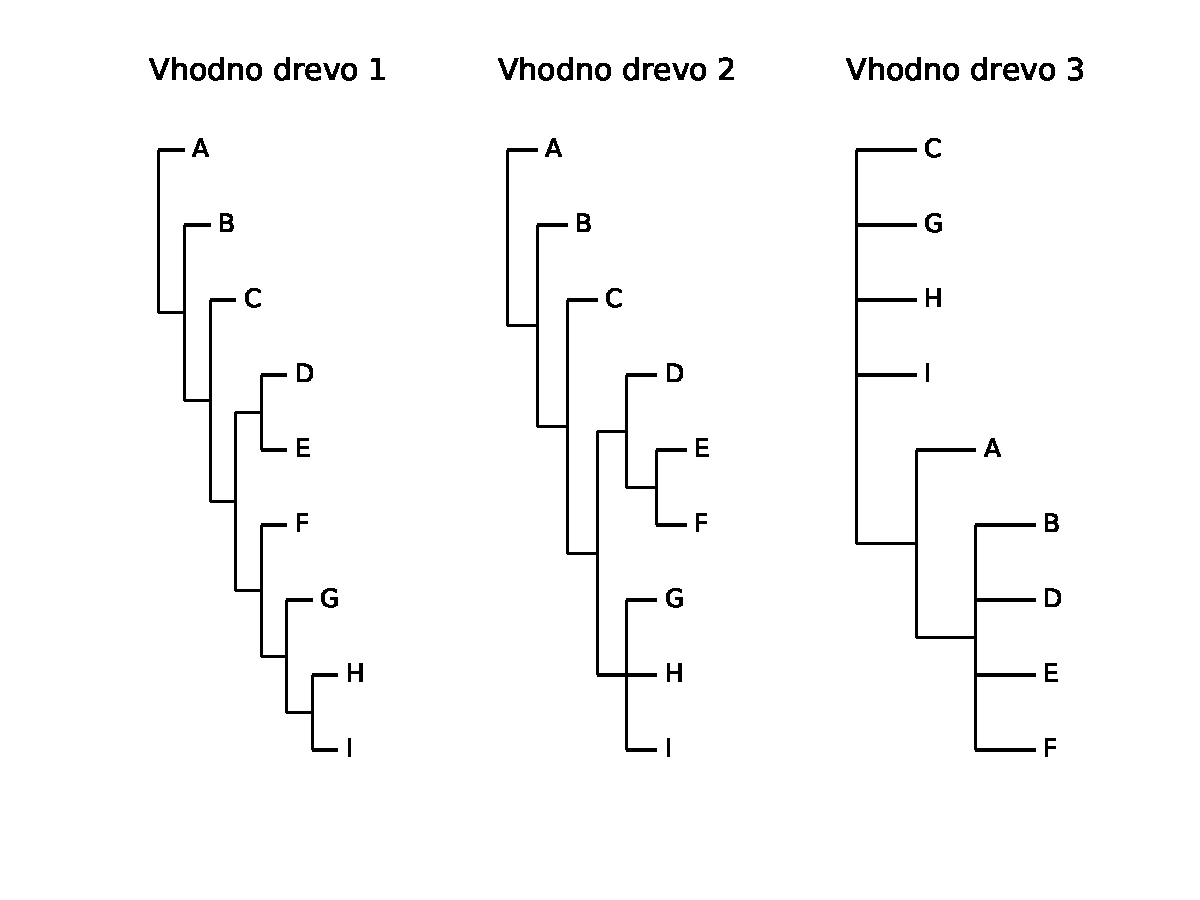
\includegraphics[scale=0.45, clip=true, trim=1cm 2cm 1cm 0]{gfx/eval_input.pdf}
	\end{center}
	\caption{Prva vhodna množica dreves.}
	\label{img-eval-input}
\end{figure}

\begin{table}
	\begin{center}
	{\footnotesize
	\begin{tabular}{ l| l | l | l | l | l }
	~                & Res ($T$) & RF ($T_1$) & RF ($T_2$) & RF ($T_3$) & RF (vsota) \\ \hline
	AMT              & 17          & 4             & 1             & 8             & 13         \\ \hline
	Bi-AMT           & 16          & 5             & 0             & 7             & 12         \\ \hline
	MM-AMT           & 13          & 3             & 4             & 5             & 12         \\ \hline
	Striktni konsenz & 10          & 6             & 5             & 2             & 13         \\ \hline
	Večinski konsenz & 17          & 2             & 5             & 4             & 11         \\ \hline
	Adamov konsenz   & 11          & 5             & 6             & 1             & 12         \\ \hline
	\end{tabular}
	\label{table-eval-1}
	\caption{Razrešenost konsenznih dreves in njihove vrednosti RF za vhodna drevesa na sliki \ref{img-eval-input}.}
	}
	\end{center}		
\end{table}

Tabela \ref{table-eval-1} prikazuje razrešenost in vrednosti RF asimetričnega
srednjega drevesa, dveh aproksimiranih asimetričnih srednjih dreves 
(Bi-AMT in MM-AMT), striktnega, večinskega in adamovega konsenznega drevesa iz 
slike~\ref{img-eval-result} glede na vhodna drevesa iz slike~\ref{img-eval-input}. 
Opazimo, da je asimetrično srednje drevo glede na razrešenost prav tako dobro 
kot večinsko konsenzno drevo. Obe drevesi sta polno razrešeni. Glede na
vrednosti RF je vhodnim drevesom najbolj podobno večinsko konsenzno drevo. 
Tako lahko brez dvoma večinsko konsenzno drevo v tem primeru razglasimo za 
najboljše.

\begin{figure}[h!]
	\begin{center}
		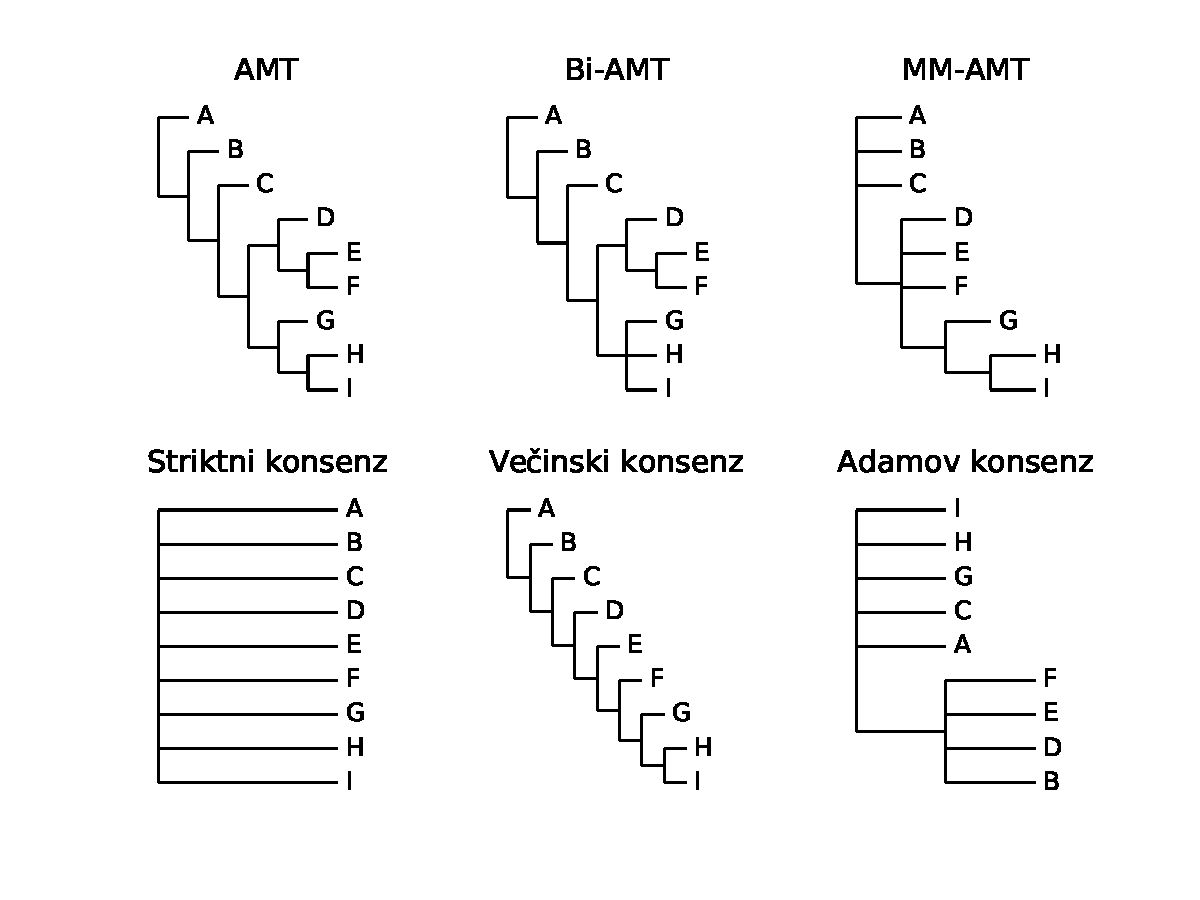
\includegraphics[scale=0.55, clip=true, trim=1.5cm 1.5cm 1cm 0.8cm]{gfx/eval_gfx.pdf}
	\end{center}
	\caption{
	         Konsenzna drevesa, zgrajena iz množice dreves na sliki \ref{img-eval-input}. Oznaka Bi-AMT označuje 
	         približek asimetričnega srednjega drevesa zgrajenega iz dveh vhodnih dreves, MM-AMT pa aproksimirano 
	         drevo zgrajeno s pomočjo največjega ujemanja.
	    }
	\label{img-eval-result}
\end{figure}

Rezultat je pričakovan, saj je večina kladov prisotnih v več kot polovici vhodnih 
dreves, preostali pa so povečini medsebojno kompatibilni, kar je za večinsko drevo
ugodno. Najbolj podobno asimetrično srednje drevo je MM-AMT, vendar je njegova 
razrešenost med najslabšimi. Drevo Bi-AMT ne podaja informacije o skupnem predniku 
taksonomskih enot $H$ in $I$, zaradi česar je bolj podobno drugemu in tretjemu 
vhodnemu drevesu kot drevo AMT, posledično pa je njegova razrešenost zaradi tega slabša. 

\section{Vhodna množica 2}
\begin{figure}[h!]
	\begin{center}
		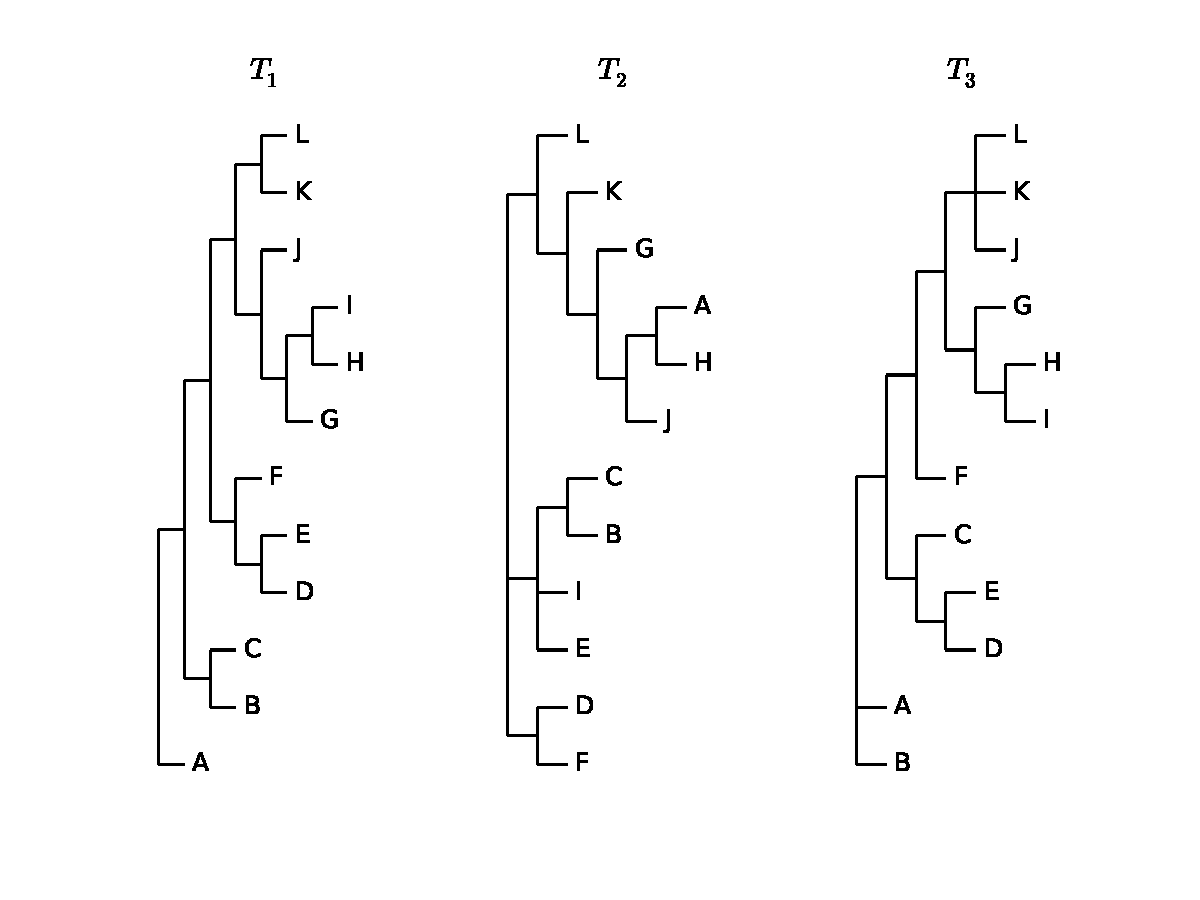
\includegraphics[scale=0.50, clip=true, trim=1cm 2cm 1cm 0]{gfx/eval_input_2.pdf}
	\end{center}
	\caption{Druga vhodna množica dreves.}
	\label{img-eval-input-2}
\end{figure}

\begin{table}[h!]
	\begin{center}
	{\footnotesize
	\begin{tabular}{ l| l | l | l | l | l }
	~                & Res ($T$) & RF ($T_1$) & RF ($T_2$) & RF ($T_3$) & RF (vsota) \\ \hline
	AMT              & 23          & 12            & 9             & 7             & 28         \\ \hline
	Bi-AMT           & 21          & 9             & 10            & 8             & 27         \\ \hline
	MM-AMT           & 14          & 10            & 9             & 7             & 26         \\ \hline
	Striktni konsenz & 15          & 7             & 8             & 8             & 23         \\ \hline
	Večinski konsenz & 23          & 10            & 11            & 9             & 30         \\ \hline
	Adamov konsenz   & 17          & 13            & 10            & 8             & 31         \\ \hline
	\end{tabular}
	\label{table-eval-2}
	\caption{Razrešenost konsenznih dreves in njihove vrednosti RF za vhodna drevesa na sliki \ref{img-eval-input-2}.}
	}
	\end{center}		
\end{table}



Rezultati konsenznih dreves iz slike \ref{img-eval-result-2} glede na vhodna 
drevesa iz slike \ref{img-eval-input-2} so prikazani v tabeli \ref{table-eval-2}. 
Ponovno sta asimetrično srednje drevo ter večinsko konsenzno drevo polno 
razrešeni. Če ti dve drevesi medsebojno primerjamo še po podobnosti vhodnim 
drevesom, se je najbolje odrezalo asimetrično srednje drevo. Nekoliko slabše 
razrešeno je drevo Bi-AMT, ki je sicer glede na metriko RF nekoliko bolj 
podobno vhodnim drevesom kot asimetrično srednje drevo. Drevo MM-AMT je sicer
po podobnosti še boljše, vendar je manj podobno in za povrh še manj razrešeno
kot striktno konsenzno drevo. Adamovo konsenzno drevo je kljub slabši razrešenosti
najmanj podobno vhodnim drevesom.

\begin{figure}[h!]
	\begin{center}
		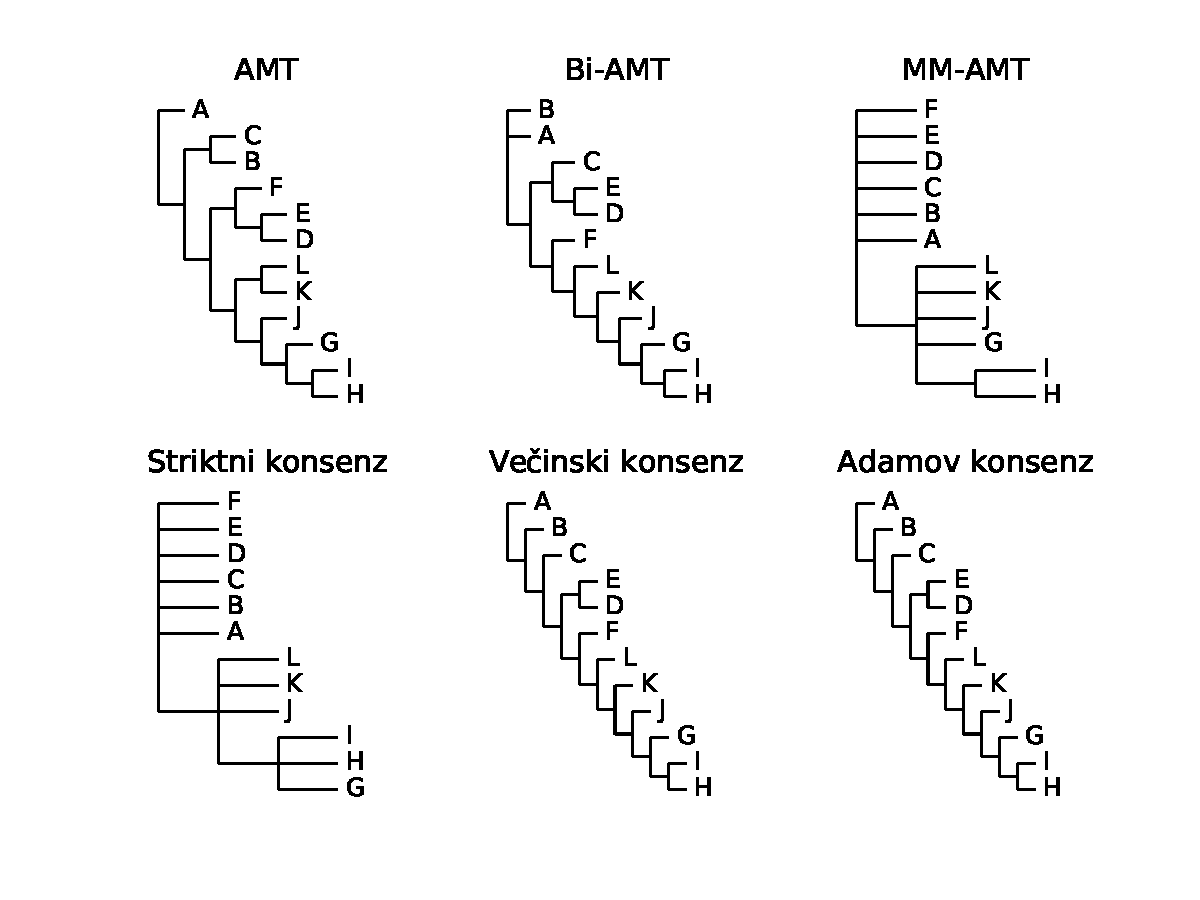
\includegraphics[scale=0.64, clip=true, trim=1.5cm 1.5cm 1cm 0.8cm]{gfx/eval_gfx_2.pdf}
	\end{center}
	\caption{Konsenzna drevesa, zgrajena iz množice dreves na sliki \ref{img-eval-input-2}.}
	\label{img-eval-result-2}
\end{figure}

Ker večina kladov ni prisotnih v več kot polovici vhodnih dreves, povečini pa so 
medsebojno kompatibilni, je rezultat pričakovan. Slaba razrešenost drevesa MM-AMT 
je najverjetneje posledica majhnega števila skupnih kladov in majhnega števila
vhodnih dreves. 

\section{Vhodna množica 3}
\begin{figure}[h!]
	\begin{center}
		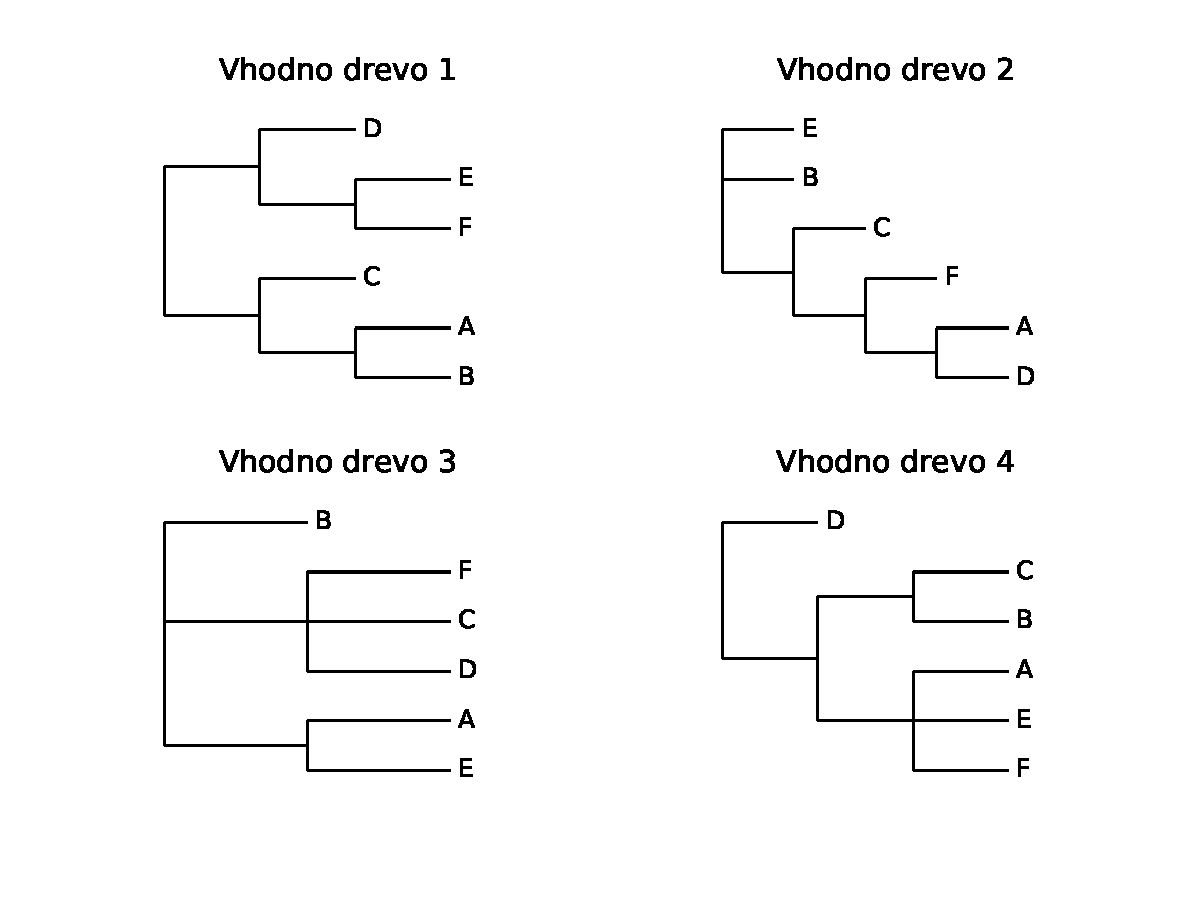
\includegraphics[scale=0.63, clip=true, trim=0 2cm 0 0.5cm]{gfx/eval_input_3.pdf}
	\end{center}
	\caption{Tretja vhodna množica dreves.}
	\label{img-eval-input-3}
\end{figure}

Tretja vhodna množica dreves iz slike \ref{table-eval-3}, je sestavljena tako, 
da je število skupnih kladov majhno, posamezni kladi ne nastopajo v več kot 
polovici vhodnih dreves in so večinoma medsebojno nekompatibilni. Rezultate
dobljenih konseznih dreves na sliki \ref{img-eval-input-3} prikazuje tabela~\ref{table-eval-3}.

\begin{table}[h!]
	\begin{center}
	{\footnotesize
	\begin{tabular}{ l| l | l | l | l | l | l }
	~                & Res (T)      & RF ($T_1$) & RF ($T_2$)       & RF ($T_3$) & RF($T_4$) & RF (vsota) \\ \hline
	AMT              & 11          & 0          & 2                & 3          & 1         & 6          \\ \hline
	Bi-AMT           & 11          & 0          & 2                & 3          & 1         & 6          \\ \hline
	MM-AMT           & 7           & 3          & 3                & 2          & 2         & 10         \\ \hline
	Striktni konsenz & 7           & 3          & 3                & 2          & 2         & 10         \\ \hline
	Večinski konsenz & 10          & 0          & 2                & 3          & 1         & 6          \\ \hline
	Adamov konsenz   & 7           & 3          & 3                & 2          & 2         & 10         \\ \hline
	\end{tabular}
	\label{table-eval-3}
	\caption{Razrešenost konsenznih dreves in njihove vrednosti RF za vhodna drevesa na sliki \ref{img-eval-input-3}.}
	}
	\end{center}		
\end{table}

Opazimo, da sta polno razrešeni le asimetrično srednje drevo in aproksimirano 
drevo Bi-AMT. Vsa ostala drevesa vsebujejo vsaj eno nerazrešeno vozlišče. 
Drevo MM-AMT je v tem primeru enako striktnemu konsenznemu drevesu in adamovem 
konsenznem drevesu, tako po topologiji kot glede na razrešenost in metriko RF. 
Preostala drevesa so glede na metriko RF sicer enakovredna, vendar ker drevo 
večinskega konsenza ni polno razrešeno, lahko za najboljši drevesi razglasimo 
asimetrično  srednje drevo in Bi-AMT drevo, ki sicer nimata popolnoma enakih 
topologij.

Slaba razrešenost drevesa MM-AMT je ponovno posledica majhnega števila skupnih
kladov in v takem primeru je aproksimacija Bi-AMT boljša. Ker posamezni kladi 
ne nastopajo v več kot polovici vhodnih dreves, metodama striktnega in adamovega 
konsenza ni uspelo popolnoma razrešiti vseh vozlišč vhodnih dreves, saj so kladi 
s premalo pojavitvami kaznovani. Asimetrično srednje drevo za razliko take klade
vključi, če to doprinese k informiranosti drevesa.

\begin{figure}
	\begin{center}
		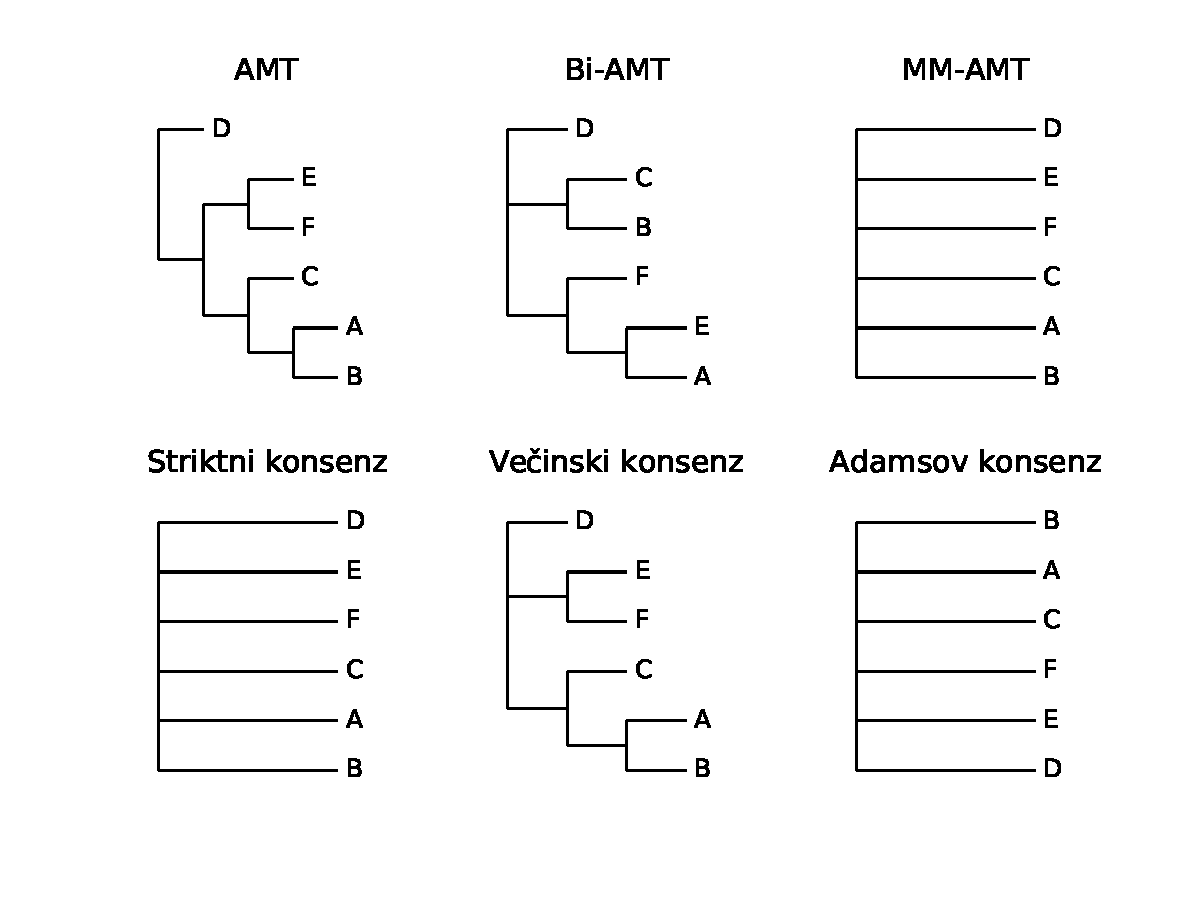
\includegraphics[scale=0.6, clip=true, trim=1.5cm 1.5cm 1cm 0.8cm]{gfx/eval_gfx_3.pdf}
	\end{center}
	\caption{Konsenzna drevesa, zgrajena iz množice dreves na sliki \ref{img-eval-input-3}.}
	\label{img-eval-result-3}
\end{figure}

Razlika med asimetričnim srednjim drevesom in aproksimiranim drevesom Bi-AMT ni 
tako očitna, ker je vhodna množica majhna. Drevo Bi-AMT je namreč zgrajeno le 
iz dveh vhodnih dreves in v kolikor bi vhodno množico povečali, bi postale razlike 
bolj očitne, saj bi bilo asimetrično srednje drevo za razliko od približka sposobno
vključiti informacije iz večih dreves hkrati.

\section{Primer puščavskih zelenih alg}
Zadnjo vhodno množico predstavlja deset dreves s 150 taksonomskimi enotami iz 
zbirke primerov programa HashCS~\cite{hashcs}. Zbirka je sicer bila zgrajena 
za potrebe uvrstitve devetih prej še neobjavljenih sekvenc puščavskih zelenih alg.
Poleg njih vsebuje še štirinajst znanih puščavskih zelenih alg in 127 taksonomskih 
enot prisotnih v tekoči vodi, morski vodi ali tleh. Drevesa so bila zgrajena s 
pomočjo programa MrBayes z uporabo GTR evolucijskega modela. Poravnane sekvence, 
ki so bile vhod v metodo bayesove inference, so bile dolge 1651 baznih parov~\cite{taxa150}.

\begin{table}[h!]
	\begin{center}
	{\footnotesize
	\begin{tabular}{ l| l | l | l | l | l | l }
	
	~            & AMT  & Bi-AMT & MM-AMT  & Striktni k. & Večinski k. & Adamov k. \\ \hline
	Res($T$)     & 298  & 279    & 242     & 151         & 284         & 259       \\ \hline
	RF($T_1$)    & 238  & 233    & 206     & 147         & 220         & 225       \\ \hline
	RF($T_2$)    & 260  & 255    & 204     & 147         & 232         & 215       \\ \hline
	RF($T_3$)    & 252  & 251    & 218     & 147         & 244         & 231       \\ \hline
	RF($T_4$)    & 258  & 243    & 190     & 147         & 248         & 233       \\ \hline
	RF($T_5$)    & 248  & 245    & 208     & 147         & 234         & 219       \\ \hline
	RF($T_6$)    & 258  & 229    & 206     & 147         & 232         & 221       \\ \hline
	RF($T_7$)    & 266  & 216    & 216     & 147         & 242         & 233       \\ \hline
	RF($T_8$)    & 256  & 241    & 212     & 147         & 242         & 221       \\ \hline
	RF($T_9$)    & 250  & 243    & 196     & 147         & 232         & 231       \\ \hline
	RF($T_{10}$) & 260  & 233    & 212     & 147         & 232         & 213       \\ \hline
	RF (vsota)   & 2546 & 2389   & 2068    & 1470        & 2358        & 2242      \\ \hline
	Čas [s]      & 164  & 293    & 11.5    & 0.3         & 3.5         & 15        \\ \hline 
	\end{tabular}
	\label{table-eval-alge}
	\caption{
	 Razrešenost konsenznih dreves in njihove vrednosti RF za deset filogenetskih dreves
	 s 150 taksonomskimi enotami~\cite{taxa150}.
	 }
	}
	\end{center}		
\end{table}
\clearpage
Rezultati v tabeli \ref{table-eval-alge} kažejo, da je najbolje razrešeno asimetrično
srednje drevo. Sledita mu večinsko konsenzno drevo in aproksimirano drevo Bi-AMT. 
Striktno konsenzno drevo je sicer najbolj podobno vhodnim drevesom, vendar najslabše 
razrešeno. Opazimo, da so vsa drevesa do neke mere žrtvovala podobnost za razrešenost
(z izjemo drevesa Bi-AMT, ki je slabše razrešeno in manj podobno vhodnim drevesom kot
večinsko). V tem smislu je metoda striktnega konsenza najbolj konzervativna, 
metoda asimetričnega srednjega drevesa pa najbolj drzna in s tem podaja največ informacij 
o evolucijskih dogodkih. 

Časovno se je najbolje odrezala metoda striktnega konsenza, sledi pa ji metoda večinskega
konsenza. Aproksimacijska metoda MM-AMT je bila hitrejša od Adamsovega konsenza,
najpočasnejša pa je bila metoda Bi-AMT.

\section{Primerjava izvajalnih časov}
Zaradi eksponentne časovne kompleksnosti metode asimetričnega srednjega drevesa nas 
zanima, kako velika drevesa in vhodne množice lahko še obdelamo v doglednem času.
Merjenje časa izvajanja smo opravili za natančno metodo, obe aproksimacijski metodi
in tudi natančno metodo z nameščenim programom PMC.   

Zgornji graf na sliki~\ref{img-eval-timing-trees} prikazuje čase izvajanja za
drevesa, ki imajo dvajset taksonomskih enot. Opazimo, da se čas izvajanja z 
večanjem števila vhodnih dreves za natančno metodo AMT povečuje zelo hitro. Preostale
metode s takimi drevesi nimajo večjih težav. Spodnji del slike prikazuje graf za
drevesa s 50 taksonomskimi enotami. Opazimo, da natančna metoda s pomočjo programa
PMC brez težav opravi z manjšimi vhodnimi množicami dreves,
nato pa prične čas naraščati precej hitreje. Čas, potreben za izvedbo aproksimacijskih 
metod tudi z večanjem števila vhodnih dreves pri večjem številu 
taksonomskih enot narašča polinomsko. Metoda Bi-AMT je kljub hitrejšemu naraščanju
izvajalnega časa za manjše število taksonomskih enot pri večjem številu taksonomskih 
enot hitrejša od metode MM-AMT. 

\clearpage
\begin{figure}[h!]
	\begin{center}
		\fbox{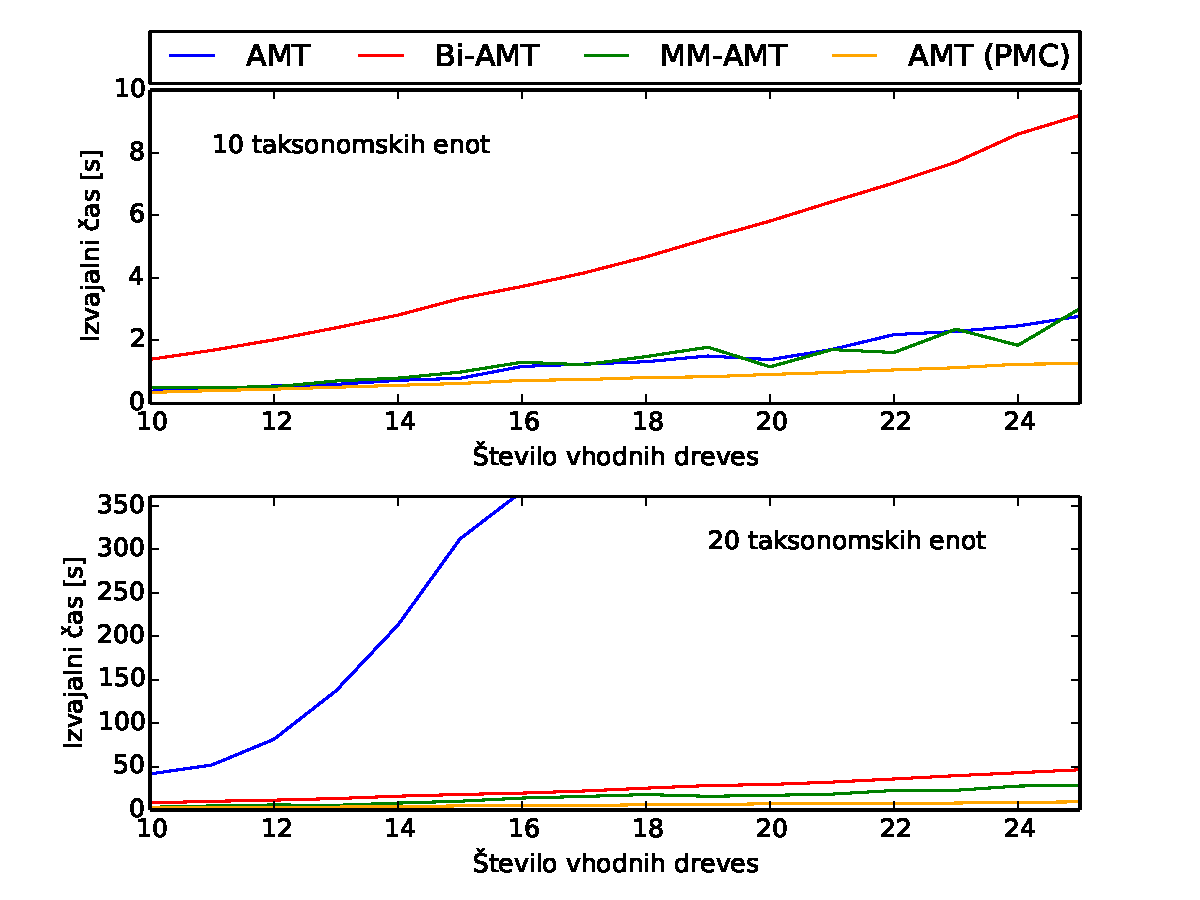
\includegraphics[scale=0.53, clip=true, trim=0 0 0 0.5cm]{gfx/times_10_20.pdf}}
	\end{center}
	\caption{
		Izvajalni časi vseh treh metod za drevesa z 20 in 50 taksonomskimi enotami
	 	za vse tri implementirane metode izračuna asimetričnega srednjega drevesa. 
	}
	\label{img-eval-timing-trees}
\end{figure}
\begin{figure}[h!]
	\begin{center}
		\fbox{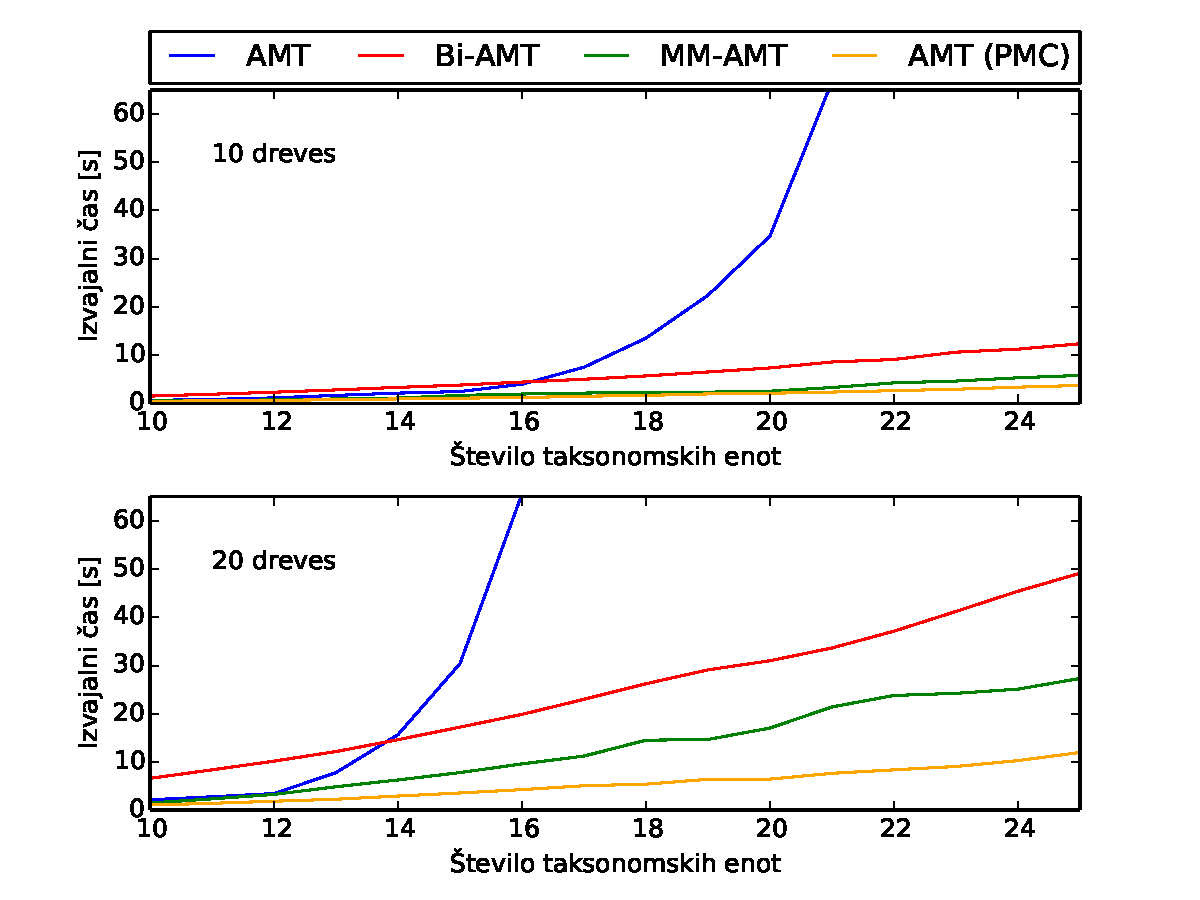
\includegraphics[scale=0.54, clip=true, trim=0 0 0 0.5cm]{gfx/times_10_20_taxons.pdf}}
	\end{center}
	\caption{
		Izvajalni časi vseh treh metod za vhodne množice 10 ali 20 dreves.
	 }
	\label{img-eval-timing-taxons}
\end{figure}

%{\bf TODO: Grafi so zelo fajn. Bi bilo pa vseeno dobro izpisati tudi
%tabelo. Predvsem, da se vidi čase izvajanja (AMT, modra linija), ki zdaj
%niti ne morejo biti prikazani, ne da bi zaradi tega stisnili ostale tri
%grafe preveč skupaj.}

Slika~\ref{img-eval-timing-taxons} prikazuje grafa časov izvajanja glede na število 
taksonomskih enot pri fiksnem številu dreves. Zgornji graf  prikazuje izvajalne čase
za deset vhodnih dreves, drugi pa za dvajset. Pri obeh so razmerja enaka. Potreben čas
za izvedbo natančne metode skokovito poraste, medtem ko čas izvajanja preostalih 
metod narašča precej počasneje. Najhitrejši je izračun točnega asimetričnega srednjega 
drevesa s pomočjo programa PMC.

Iz zgornjih grafov je razvidno, da na čas izvajanja bistveno bolj kot število taksonomskih
enot vpliva število vhodnih dreves. Vendar ni tako enostavno. Zaradi naključnega generiranja 
dreves vhodne množice težko trdimo, kakšne so bile njihove lastnosti.  Število 
taksonomskih enot v drevesu je neposredno povezano z globino drevesa. V kolikor
je taksonomskih enot več, potem je število možnih poddreves večje. Z večjim številom
možnih poddreves se poveča tudi število potencialnih vozlišč v grafu nekompatibilnosti.
Slednje je sicer odvisno tako od števila dreves v vhodni množici kot njihovih lastnosti.
Drevesa lahko vsebujejo veliko število taksonomskih enot, a so si medsebojno precej
podobna, pri čemer bo graf nekompatibilnosti majhen, četudi je število vhodnih dreves 
zelo veliko, in posledično bo čas izvajanja krajši. Na drugi strani število taksonomskih 
enot ne rabi biti zelo veliko, da naletimo na težave s časom izvajanja, če so drevesa 
medsebojno zelo različna.

Zaključimo torej lahko, da je izračun asimetričnega srednjega drevesa s pomočjo natančne
metode za večje vhodne množice smotrn le z uporabo
zunanjega programa PMC. Tudi tu sicer naletimo na težave, vendar precej pozneje. Primer 
puščavskih zelenih alg, ki vsebuje 150 taksonomskih enot in deset dreves, smo naprimer 
uspeli izračunati v dvajsetih minutah, medtem ko so naključno generirani primeri 
pokazali, da v splošnem čas, potreben za izračun, lahko skokovito naraste. Ocenimo
lahko, da je uporaba natančne metode izračuna trenutno smotrna za srednje velike 
vhodne podatke s 150 taksonomskimi enotami in do 50 drevesi, dejanske številke pa so odvisne od
lastnosti vhodnih dreves. V primeru težav lahko posežemo po aproksimacijskih metodah, 
kjer na težave s časom izvajanja nebi smeli naleteti.

\chapter{Zaključek}
Najpomembnejši rezultat dela je zagotovo prva znana implementacija konsenzne metode
asimetričnega srednjega drevesa v programski paket Biopython. Čeprav je računska 
kompleksnost metode v splošnem eksponentna (sliki~\ref{img-eval-timing-trees} 
in~\ref{img-eval-timing-taxons}), kar je nezaželjeno, in se problemi z
izvajalnim časom za natančno metodo pojavijo hitro, ima uporabnik možnost namestitve 
zunanjega programa PMC, ki bistveno pospeši izvajanje. Kljub temu je za velike vhodne 
množice dreves izračun lahko dolgotrajen, čeprav to ne velja v splošnem,
saj lastnosti vhodnih dreves (število kompatibilnih poddreves) igrajo velik faktor pri
iskanju največje neodvisne množice, ki je računsko najintenzivnejši del. V kolikor 
uporabnik naleti na težave s časom izvajanja, lahko izbere eno izmed 
aproksimacijskih metod, katerih časovna zahtevnost le manjša. Pravilna izbira 
aproksimacijske metode je, kot smo pokazali tudi eksperimentalno, odvisna 
predvsem od lastnosti dreves v vhodni množici. 

Kot smo pokazali na štirih vhodnih množicah, asimetrično srednje drevo ni nujno 
tisto, ki drevesa vhodne množice glede na Robinson-Fouldsovo metriko povzema 
najbolje. Prav tako kot pri izbiri aproksimacijske metode tudi tukaj velja, da 
je izbira konsenzne metode odvisna predvsem od predhodnega poznavanja lastnosti 
dreves vhodne množice. V kolikor ta vsebujejo veliko število nekompatibilnih parov 
poddreves, potem je izbira metode asimetričnega srednjega drevesa smotrna, v 
nasprotnem primeru pa lahko že večinsko konsenzno drevo da primerljive, če ne 
celo boljše rezultate.

Kar se tiče razrešenosti dreves, smo na realnem in nekaj umetnih primerih pokazali, da 
je asimetrično srednje drevo vedno bilo najbolje razrešeno in tako ponujalo največ 
informacij o evolucijski zgodovini, s čimer je prekašalo vse ostale metode. 
Tega sicer ne moremo trditi za obe aproksimacijski metodi. Metoda z izračunom 
največjega ujemanja je po razrešenosti v nekaterih primerih bila primerljiva zgolj 
s striktnim konsenznim drevesom, v drugih pa je bila nekoliko boljša od adamovega 
konsenznega drevesa. Metoda z izračunom drevesa iz dveh vhodnih dreves je ob 
primerljivi razrešenosti glede na večinsko konsenzno drevo običajno proizvedla drevo,
ki se slabše ujema z vhodnimi drevesi. 

Možnosti za izboljšave vidimo predvsem pri aproksimacijskih algoritmih. Nad drevesi,
izračunanimi s pomočjo prvega aproksimacijskega algoritma, bi npr. lahko ponovno 
izračunali konsenzna drevesa in izbrali najboljšega. Poleg tega bi lahko
izračun asimetričnega srednjega drevesa za vsak par vhodnih dreves opravili paralelno. 

Eksponentni čas za konstrukcijo asimetričnega srednjega drevesa bi lahko zmanjšali z 
uporabo katerega izmed aproksimacijskih algoritmov za iskanje največje neodvisne množice.
Prav tako bi bilo zanimivo določiti lastnosti množice vhodnih dreves, za katero da 
metoda asimetričnega srednjega drevesa boljše rezultate od ostalih konsenznih metod.

\addcontentsline{toc}{chapter}{Literatura}
\begin{thebibliography}{99}

\bibitem{cd}
C.\ Darwin. ``Notebook B: Transmutation of species'', str. 36, 1837-1838.

\bibitem{pw}
C.\ Phillips, T.\ J.\ Warnow. 
``The asymmetric median tree - A new model for building consensus trees'', 
{\it Discrete Applied Mathematics}, št.\ 71, str.\ 311–335, 1996.

\bibitem{classification}
D.\ Bryant. ``A classification of consensus methods for phylogenetics.'', 
{\it Bioconsensus}, str. 163–185.

\bibitem{gd}
D. Gusfeld. ``Efficient algorithms for inferring evolutionary trees'', 
{\it Networks}, št. 21, str.\ 19-28, 1991.

\bibitem{fel}
J.\ Felsenstein. \textit{Inferring Phylogenies}. Sinauer Associates, 2004.

\bibitem{fel-ml}
J.\ Felsenstein. ``Evolutionary Trees from DNA Sequences: A Maximum Likelihood Approach'', 
{\it Journal of Molecular Evolution}, št. 17, str. 368-376, 1981.

\bibitem{bw}
T.\ Y.\ Berger-Wolf. 
``Properties of compatibility and consensus sets of phylogenetic trees''. 
{\it UNM Computer Science Technical Report}, TR-CS-2004-24, 2004.

\bibitem{rf}
T.\ Asano, J.\ Jansson, K.\ Sadakane, R.\ Uehara, G.\ Valiente. 
``Faster computation of the Robinson–Foulds distance between phylogenetic networks'', 
{\it Information Sciences}, št. 197, str.\ 77-90, 2012.

\bibitem{jc}
T.\ H.\ Jukes, C.\ R.\ Cantor. ``Evolution of protein molecules'', 
{\it Mammalian protein metabolism}, št. 3, str.\ 21-132, 1969.

\bibitem{k80}
M.\ Kimura. 
``A Simple Method for Estimating Evolutionary Rates of Base Substitutions 
Through Comparative Studies of Nucleotide Sequences'', 
{\it Journal of Molecular Evolution}, št. 16, str.\ 111-120, 1980.

\bibitem{clustalw2}
M.\ A.\ Larkin, G.\ Blackshields, N.\ P.\ Brown, R.\ Chenna, 
P.\ A.\ McGettigan, H.\ McWilliam, F.\ Valentin, I.\ M.\ Wallace, 
A.\ Wilm, R.\ Lopez, J.\ D.\ Thompson,
T.\ J.\ Gibson, D.\ G.\ Higgins. 
``ClustalW and ClustalX version 2'', 
{\it Bioinformatics}, št. 23, str. 2947–2948, 2007.

\bibitem{phylip}
J.\ Felsenstein. {\it PHYLIP (Phylogeny Inference Package) version 3.6}. 
Department of Genome Sciences, University of Washington, Seattle.

\bibitem{gtr}
S.\ Tavare. 
``Some probabilistic and statistical problems in the analysis of DNA sequences.'', 
{\it Lectures on Mathematics in the Life Sciences}, št. 17, str.\ 57-86,  1986.

\bibitem{parsimony}
P.\ Lemey, M.\ Salemi, A.\ Vandamme. 
{\it The Phylogenetic Handbook: a Practical Approach to Phylogenetic Analysis 
and Hypothesis Testing}. 
Cambridge University Press, 2009.

\bibitem{mrbayes}
F.\ Ronquist, M.\ Teslenko, P.\ van der Mark, D.\ L.\ Ayres, A.\ Darling, 
S.\ Höhna, B.\ Larget, L.\ Liu, M.\ A.\ Suchard, J.\ P.\ Huelsenbeck. 
``MrBayes 3.2: Efficient Bayesian Phylogenetic Inference and Model 
Choice Across a Large Model Space'', 
{\it Systematic Biology}, 
št. 61, str.\ 539-542, 2012.

\bibitem{mega6}
K.\ Tamura, G.\ Stecher, D.\ Peterson, A.\ Filipski, S.\ Kumar. 
``MEGA6: Molecular Evolutionary Genetics Analysis Version 6.0'', 
{\it Molecular biology and evolution}, 
št. 30, str. 2725–2729, 2013.

\bibitem{biopython}
P.\ J.\ A.\ Cock, T.\ Antao, J.\ T.\ Chang, B.\ A.\ Chapman, 
C.\ J.\ Cox, A.\ Dalke, I.\ Friedberg, T.\ Hamelryck, 
F.\ Kauff, B.\ Wilczynwski, M.\ J.\ L.\ de Hoon.
``Biopython: freely available Python tools for computational 
molecular biology and bioinformatics'', 
{\it BMC Bioinformatics}, 
str. 1422-1423, št. 11, 2009.

\bibitem{bio-phylo}
E.\ Talevich, B.\ M.\ Invergo, P.\ J.\ A.\ Cock, B.\ A.\ Chapman.
``Bio.Phylo: A unified toolkit for processing, analyzing and 
visualizing phylogenetic trees in Biopython'', 
{\it BMC Bioinformatics}, 
št. 13, 2012.

\bibitem{hashcs}
S.\ S.\ Sul, T.\ L.\ Williams. 
``An Experimental Analysis of Consensus Tree Algorithms for 
Large-Scale Tree Collections'', 
{\it 5th Intl. Symposium on Bioinformatics Research and Applications}, 
str. 100-111, 2009.

\bibitem{pmc}
R.\ A.\ Rossi, D.\ F.\ Gleich, A.\ H.\ Gebremedhin, M. M.\ Patwary.  
``A Fast Parallel Maximum Clique Algorithm for Large Sparse Graphs 
and Temporal Strong Components'', 
{\it arXiv preprint 1302.6256}, 2013.  

\bibitem{taxa150}
L.\ A.\ Lewis, P.\ O.\ Lewis. 
``Unearthing the Molecular Phylodiversity of Desert Soil Green Algae (Chlorophyta)'', 
{\it Systematic Biology}, 
št. 54, str. 936-947, 2005.

\bibitem{hopcroft-karp}
J.\ E.\ Hopcroft, R.\ M.\ Karp. 
``An $n^{\frac{5}{2}}$ Algorithm for Maximum Matchings in Bipartite Graphs''. 
{\it SIAM Journal on Computing}, 
str. 225-231, št. 4, 1973.

\bibitem{phy} 
Phylogenetics,
dostopno na:\\ http://en.wikipedia.org/wiki/Phylogenetics

\bibitem{mgt}
Matching (Graph Theory),
dostopno na: \\ http://en.wikipedia.org/wiki/Matching\_(graph\_theory)


\end{thebibliography}

\newpage
\appendix
\chapter{Testna programska koda \label{appendix-code-metrics}}

\begin{python}
from Bio import Phylo
from Bio.Phylo import Consensus as cons
import dendropy
from matplotlib import pyplot

trees = list(Phylo.parse('vhodna_drevesa.tre', 'newick'))
amts = {
    'AMT': cons.amt_consensus(trees, method='no_approx'),
    'Bi-AMT': cons.amt_consensus(trees, method='bi_approx'),
    'MM-AMT': cons.amt_consensus(trees, method='maxmatch_approx')
}
other = {
    'Strict': cons.strict_consensus(trees),
    'Majority': cons.majority_consensus(trees),
    'Adam': cons.adam_consensus(trees)
}

def _plot(nx, ny, fig, i, tree, title):
    ax = fig.add_subplot(ny, nx, i)
    fig.subplots_adjust(wspace=0.5)
    Phylo.draw(tree, do_show=False, axes=ax)
    pyplot.axis('off')
    pyplot.title(title)

# Shrani vhodna drevesa v datoteke
for i, tree in enumerate(trees):
    Phylo.write(tree, 'eval/in_%d.tre' % i, 'newick')

# Shrani konsenzna drevesa v datoteke
for name, tree in amts.items() + other.items():
    tree.ladderize()
    Phylo.write(tree, 'eval/%s.tre' % name, 'newick')

# Izrisi vhodna drevesa v datoteko input_trees.pdf
input_trees = pyplot.figure(0)
x = len(trees)
for i, t in enumerate(trees):
    _plot(x, 1, input_trees, i, t, 'Vhodno drevo %d' % i)
pyplot.savefig('input_trees.pdf')

# Izrisi konsenzna drevesa v datoteko consensus_trees.pdf
output_trees = pyplot.figure(1)
for i, kt in enumerate(amts.items() + other.items()):
    k, t = kt
    _plot(3, 2, output_trees, i, t, k)
pyplot.savefig('consensus_trees.pdf')

# Nalozi drevesa z DendroPy
d_amts = {
    k: dendropy.Tree(stream=open('eval/%s.tre' % k), schema='newick')
    for k in amts.keys()
}
d_other = {
    k: dendropy.Tree(stream=open('eval/%s.tre' % k), schema='newick')
    for k in other.keys()
}
d_input = [
    dendropy.Tree(stream=open('eval/in_%d.tre' % i), schema='newick')
    for i in range(0, len(trees))
]

tpl = '[{0:10}] Res = {1:4} RF_sum: {2:5} RFs: {3}'
for k in d_amts.keys() + d_other.keys():
    if k in d_amts:
        t = d_amts[k]
    else:
        t = d_other[k]

    diffs = []
    total_diff = 0
    edges = len(t.get_edge_set())
    t.is_rooted = False
    t.update_splits()
    for in_tree in d_input:
        if in_tree.is_rooted:
            in_tree.is_rooted = False
            in_tree.update_splits()
        d = in_tree.symmetric_difference(t)
        diffs.append(str(d))
        total_diff += d

    print tpl.format(k, edges, ','.join(diffs), total_diff)
\end{python}
% fake figure ^^
\begin{figure}[h!]
	\label{app-code-metrics}
	\footnotesize
	{
	\caption{
		Testna programska koda za merjenje razrešenosti konsenznih dreves 
		in Robinson-Fouldsove metrike. Koda naloži vhodno množico dreves 
		in iz nje izračuna konsenzna drevesa s pomočjo šestih metod. 
		Nato vhodna drevesa in izračunana drevesa izriše v PDF datoteki 
		ter vsako drevo shrani v datoteko v formatu Newick. S pomočjo 
		knjižnice DendroPy nato ta drevesa naloži in nad konsenznimi drevesi 
		izračuna razrešenost ter Robinson-Fouldsovo metriko glede na 
		vsako vhodno drevo.
	}
	}
\end{figure}
\clearpage
\begin{python}
from Bio.Phylo.BaseTree import Tree
from Bio.Phylo.Consensus import amt_consensus as amt
import time

current_time = lambda: int(round(time.time() * 1000))


def _test(method, trees):
    s = current_time()
    _ = amt(trees, method=method)
    return current_time() - s

N_TAXONS = range(10, 50)
N_TREES = 10
N_ITERS = 10
METHOD = 'no_approx'

for n in N_TAXONS:
    total = 0.0
    trees = [Tree.randomized(n) for i in range(0, N_TREES)]
    for _ in range(0, N_ITERS):
        total += _test(METHOD, trees)
    print '[%s, %d taxons, %d tress]: %fms' % (METHOD, n, N_TREES, total/float(N_ITERS))
\end{python}
% fake figure ^^
\begin{figure}[h!]
	\label{app-code-time}
	\footnotesize
	{
	\caption{
		Testna programska koda za merjenje časa izvajanja. Spremenljivka 
		{\it N\_TREES} določa število dreves, ki bodo naključno generirana 
		in predstavljala vhodno množico. Nad temi drevesi nato izračunamo 
		asimetrično srednje drevo z metodo, ki jo določa spremenljivka {\it METHOD}.  
	}
	}
\end{figure}

\chapter{Programska koda metode {\it Bio.Phylo.Consensus.amt\_consensus}\label{appendix-code-amt_consensus}}

\begin{python}
def amt_consensus(trees, method='no_approx'):
  """Search Asymmetric Median Tree from multiple trees

  :Parameters:
  trees: list
      list of trees to produce consensus tree

  @type trees: list of Bio.Phylo.BaseTree.Tree
  @returns: Bio.Phylo.BaseTree.Tree
  """
  import multiprocessing
  import re
  from distutils.spawn import find_executable
  from itertools import combinations
  from scipy import io
  from scipy import sparse
  from subprocess import Popen, PIPE

  species = trees[0].get_terminals()
  species_names = [s.name for s in species]
  n_species = len(species)
  n_trees = len(trees)
  cpus = multiprocessing.cpu_count()

  def _tree_encoding(tree):
    clades = [
      bs for _, bs 
      in _tree_to_bitstrs(tree, species_names).items() 
      if bs.count('1') != n_species
    ]
    leaves = [
      _clade_to_bitstr(cld, species_names) for cld 
      in tree.find_clades(terminal=True)
    ]
    return list(set(clades + leaves))

  tree_encodings = [_tree_encoding(t) for t in trees]
  profile_bitstrings = set(reduce(
    lambda enc1, enc2: enc1 + enc2, tree_encodings
  ))
  bitstring_weights = {
    bs: len([
      i for i, t 
      in enumerate(tree_encodings) if bs in t
    ]) for bs in profile_bitstrings
  }
  common_bitstrings = set(
    bs for bs, w in bitstring_weights.items() 
    if w == n_trees
  )

  def _amt_val(tree_encoding):
    tree_enc_set = set(tree_encoding)
    if len(common_bitstrings - tree_enc_set) != 0 or len(tree_enc_set - profile_bitstrings) != 0:
      res = -float('Inf')
    else:
      res = sum([
        bitstring_weights[w] 
        for w in tree_enc_set - common_bitstrings
      ])

    return res

  def _incompat_graph_nx(trees):
    all_bs = reduce(lambda x, y: x+y, trees, [])
    unique_bitstrings = list(set(all_bs))
    incompatible_pairs = [
      (bs1, bs2) for bs1 in unique_bitstrings 
      for bs2 in unique_bitstrings 
      if not bs1.iscompatible(bs2)
    ]
    incomp_graph = nx.Graph()
    incomp_graph.add_nodes_from(unique_bitstrings)
    incomp_graph.add_edges_from(incompatible_pairs)

    return incomp_graph, unique_bitstrings

  def _max_indep_set(incomp_graph, unique_bitstrings):
    def _pmc(pmc_exec_path):
      comp_bitstrings = [
        bs for bs in unique_bitstrings 
        if bs not in common_bitstrings
      ]
      comp_graph = nx.complement(incomp_graph)
      comp_graph.remove_nodes_from(common_bitstrings)
      mtx = nx.to_numpy_matrix(comp_graph, nodelist=comp_bitstrings)
      mtx = sparse.coo_matrix(np.tril(mtx))
      io.mmwrite('/tmp/igc', mtx, field='integer')

      process = Popen([pmc_exec_path, '-f', '/tmp/igc.mtx', '-a', '0', '-t', str(cpus), '-r', '0'], stdout=PIPE)
      (output, err) = process.communicate()
      exit_code = process.wait()

      if exit_code != 0:
        raise Exception('PMC aborted... %s' % err)
      else:
       pmc_regex = re.compile('Maximum clique:\s([\d\s]*)')
       match = re.search(pmc_regex, output)
        if match is None:
          raise Exception('Couldnt find PMC output. [%s]' % output)
        elif len(match.groups()) > 2:
          pmc_out = match.group(2).split(' ')
        else:
          pmc_out = match.group(1).split(' ')
        mis_vertices = [
          comp_bitstrings[int(v)-1] for v in pmc_out 
          if v != '\n'
        ] + list(common_bitstrings)
        max_val = _amt_val(mis_vertices)
      return mis_vertices, max_val

    def _netx():
      current_max_size = 0
      comp_graph = nx.complement(incomp_graph)
      comp_graph.remove_nodes_from(common_bitstrings)
      maxes = []
      for clq in nx.find_cliques(comp_graph):
        if len(clq) > current_max_size:
          maxes = [clq]
          current_max_size = len(clq)
        elif len(clq) == current_max_size:
          maxes.append(clq)
      current_max = None
      current_best_val = -float('inf')
      for clq in maxes:
        mis = clq + list(common_bitstrings)
        val = _amt_val(mis)
        if val > current_best_val:
          current_best_val = val
          current_max = mis
      return current_max, current_best_val

    pmc_exec = find_executable('pmc')
    if pmc_exec is not None:
      return _pmc(pmc_exec)
    else:
      return _netx()

  def _reconstruct(bitstrings):
    m = np.transpose(
      np.array([
        bs.to_numpy() for bs 
        in sorted(bitstrings, 
          reverse=True, 
          key=lambda bs: int(bs)
        )
      ])
    )
    ones = np.transpose(np.nonzero(m))
    row_indices = np.unique(ones[:, 0])
    col_indices = np.unique(ones[:, 1])
    cols_by_rows_index = {
      ridx: ones[ones[:, 0] == ridx][:, 1] 
      for ridx in row_indices
    }
    column_values = {cidx: [] for cidx in col_indices}

    for cell in ones:
      cols = cols_by_rows_index[cell[0]]
      valid_cols = cols[cols < cell[1]]
      max_k = np.max(valid_cols) if valid_cols.size != 0 else None
      column_values[cell[1]].append(max_k)

    for k in column_values.keys():
      if len(set(column_values[k])) == 1:
        column_values[k] = column_values[k][0]
      else:
        raise Exception('Column %d not unique, tree does not exist for given encoding.' % k)

    nodes = {
      eid: BaseTree.Clade(name=eid) 
      for eid in column_values.keys() + ['root']
    }
    top_level_edges = [
      eid for eid in column_values.keys() 
      if column_values[eid] is None
    ]
    other_edges = [
      eid for eid in column_values.keys() 
      if column_values[eid] is not None
    ]
    # connect top level edges to root
    for eid in top_level_edges:
      nodes['root'].clades.append(nodes[eid])
    # connect other nodes between each other
    for eid in other_edges:
      nodes[column_values[eid]].clades.append(nodes[eid])
    # label terminals (tree leaves)
    max_cols_by_rows = {
      ridx: np.max(cols_by_rows_index[ridx]) 
      for ridx in cols_by_rows_index.keys()
    }
    for row_id in max_cols_by_rows:
      term = nodes[max_cols_by_rows[row_id]]
      term.name = species_names[row_id]

    # purge node names if they do not contain string or they contain 'root' string
    for nk in nodes.keys():
      if type(nodes[nk].name) != str or nodes[nk].name == 'root':
        nodes[nk].name = ''

    return BaseTree.Tree(root=nodes['root'])

  def _amt_approx_bi(trees):
    """
    Computes AMT from input trees using approximation 
    method 1 (computing AMTs from two trees at a time).
    @type trees:  list of list of _BitString
    @return: Bio.Phylo.BaseTree.Tree
    """
    best_amt = None
    best_amt_val = -float('inf')
    for comb in combinations(range(0, len(trees)), 2):
      incomp_graph, ubs = _incompat_graph_nx([
        trees[comb[0]], trees[comb[1]]
      ])
      incomp_graph.remove_nodes_from(common_bitstrings)
      verts = incomp_graph.nodes()
      top, bottom = nx.bipartite.sets(incomp_graph)
      if len(top) == 0:
        mvc = bottom
      elif len(bottom) == 0:
        mvc = top
      else:
        mates = nx.max_weight_matching(incomp_graph, maxcardinality=True)
        matched = mates.keys()
        top_unmatched = [
          v for v in top 
          if v not in matched
        ]
        cwo = [
          adj for adj in incomp_graph[v] 
          if adj in bottom 
          for v in top_unmatched
        ]
        cwo += top_unmatched
        mvc = set(
          [v for v in top if v not in cwo] 
          + list(set(bottom) & set(cwo))
        )
      mis = [v for v in verts if v not in mvc]
      bitstrings = list(common_bitstrings) + mis
      val = _amt_val(bitstrings)
      if val > best_amt_val:
        best_amt = bitstrings
        best_amt_val = val

    return _reconstruct(best_amt)

  def _amt_approx_mm(trees):
    """
    Computes AMT from input trees using approximation 
    method 2 (maximum matching)
    @type trees: list of list of _BitString
    @return Bio.Phylo.BaseTree.Tree
    """
    incomp_graph, unique_bitstrings = _incompat_graph_nx(trees)
    vertices = incomp_graph.nodes()
    incomp_graph.remove_nodes_from(common_bitstrings)
    matching = nx.max_weight_matching(incomp_graph, maxcardinality=True)
    for match in matching.keys():
      vertices.remove(match)
    return _reconstruct(vertices)

  def _amt_noapprox(trees):
    """
    Computes AMT from input trees.
    @type trees: list of list of _BitString
    @return Bio.Phylo.BaseTree.Tree
    """
    incomp_graph, unique_bitstrings = _incompat_graph_nx(trees)
    mis, mis_val = _max_indep_set(incomp_graph, unique_bitstrings)
    return _reconstruct(mis)

  if method == 'no_approx':
    amt = _amt_noapprox(tree_encodings)
  elif method == 'bi_approx':
    amt = _amt_approx_bi(tree_encodings)
  elif method == 'maxmatch_approx':
    amt = _amt_approx_mm(tree_encodings)
  else:
    raise Exception('Invalid method name. Given: %s; available: no_approx, bi_approx, maxmatch_approx' % method)

  return amt
\end{python}

\end{document}

